\documentclass[12pt,reqno]{amsart}
%\documentclass{amsart}
\renewcommand{\labelenumi}{(\alph{enumi})}



\setlength{\textwidth}{6in}
\setlength{\textheight}{8.5in}
\hoffset=-0.5in

\usepackage{diagrams}

\usepackage[utf8]{inputenc}
\usepackage{graphicx}
\usepackage{amssymb}
\usepackage{amsmath}
\usepackage{epstopdf}
\usepackage{amsthm}
\usepackage{mathrsfs}
%\usepackage{xypic}
\usepackage{enumerate}
%\usepackage{sidenotes}
\usepackage{listings}

%\usepackage{fourier}
%\usepackage{a4wide}


\newtheorem{definition}{Definition} 
\numberwithin{definition}{section}
\newtheorem{proposition}[definition]{Proposition} 
\newtheorem{theorem}[definition]{Theorem} 
\newtheorem{lemma}[definition]{Lemma} 
\newtheorem{corollary}[definition]{Corollary}
\newtheorem{conjecture}[definition]{Conjecture}
\newtheorem{question}[definition]{Question}
\newtheorem{claim}[definition]{Claim}
\newtheorem{fact}[definition]{Fact}
\newtheorem{remark}[definition]{Remark}
\newtheorem{wedgelemma}[definition]{Wedge Lemma} 
\newtheorem{construction}[definition]{Construction}

\theoremstyle{definition}
\newtheorem{example}[definition]{Example}



 \newcommand{\lo}{\preceq}
\newcommand{\rar}{\rightarrow}
\newcommand{\rAr}{\Rightarrow}
\newcommand{\lrAr}{\Leftrightarrow}
\newcommand{\RR}{\mathbb{R}}
\newcommand{\NN}{\mathbb{N}}
\newcommand{\QQ}{\mathbb{Q}}
\newcommand{\ZZ}{\mathbb{Z}}
\newcommand{\AAA}{\mathcal{A}}
\newcommand{\FFF}{\mathcal{F}}
\newcommand{\HHH}{\mathcal{H}}
\newcommand{\NNN}{\mathcal{N}}
\newcommand{\SSS}{\mathcal{S}}
\newcommand{\K}{\mathbf{K}}
\renewcommand{\L}{\mathbf{L}}
\newcommand{\U}{\mathbf{U}}
\newcommand{\V}{\mathbf{V}}
\newcommand{\X}{\mathbf{X}}
\newcommand{\Rat}{\operatorname{Rat}}
\newcommand{\cox}{\operatorname{Cox}}
\newcommand{\ehr}{\operatorname{ehr}}
\newcommand{\dist}{\mathsf{dist}}
\newcommand{\sgn}{\mathrm{sgn}}
\newcommand{\sprod}[2]{\langle #1, #2 \rangle}
\newcommand{\mspan}{\operatorname{span}}
\renewcommand{\dim}{\mathsf{dim}\ }
\newcommand{\inter}{\mathsf{int}\ }
\newcommand{\median}{\mathrm{median}\ }
\DeclareMathOperator*{\argmin}{arg\,min}

\newcommand{\defn}[1]{\emph{#1}}
\newcommand{\norm}[1]{|| #1 ||}

\newcommand{\Glat}{G^{\operatorname{lat}}}
\newcommand{\Gdep}{G^{\operatorname{dep}}}
\newcommand{\Gfine}{G^{\operatorname{fine}}}
\newcommand{\Gfinem}{G^{\operatorname{fine*}}}

\newcommand{\FD}{\mathcal{F}}

\newcommand{\path}{\operatorname{path}}
\newcommand{\reldep}[2]{{#1} \longrightarrow {#2}}
\newcommand{\reldepi}[3]{{#1} \overset{#2}{\longrightarrow} {#3}}
\newcommand{\shift}[2]{\rightarrow(#1,{#2})}
\newcommand{\shiftw}[3]{\overset{#1 \cdot #2}{\longrightarrow} {#3}}

\newcommand{\conv}{\operatorname{conv}}
\newcommand{\cone}{\operatorname{cone}}
\newcommand{\lev}{\operatorname{lev}}
\newcommand{\Lev}{\operatorname{Lev}}
\renewcommand{\deg}{\operatorname{deg}}
\renewcommand{\dim}{\operatorname{dim}}
\renewcommand{\min}{\operatorname{min}}
\renewcommand{\max}{\operatorname{max}}
\newcommand{\fract}{\operatorname{frac}}
\newcommand{\integ}{\operatorname{int}}
\newcommand{\relint}{\operatorname{relint}}
\newcommand{\type}{\operatorname{type}}

\newcommand{\twin}{\mathsf{twin}}
\newcommand{\hull}{\mathsf{hull}}
\newcommand{\diam}{\mathsf{diam}}
\newcommand{\choice}[1]{\left\{ \begin{array}{ll} #1 \end{array} \right.}
\newcommand{\floor}[1]{\lfloor {#1} \rfloor}
\newcommand{\ceil}[1]{\lceil {#1} \rceil}
\newcommand{\mset}[2]{ \left\{ #1 \; \middle| \; #2 \right\}}
\newcommand{\lk}{\mathsf{lk}}
\newcommand{\sd}{\mathsf{sd}}
\newcommand{\Pa}{\mathrm{P}}
\newcommand{\dotcup}{\ensuremath{\mathaccent\cdot\cup}}
\newcommand{\Hom}{\mathrm{ Hom}}
\newcommand{\om}{\omega}

%% IMPORTANT OBJECTS FOR THIS ARTICLE

\newcommand{\ncS}{\mathcal{S}}
\newcommand{\ncM}{\mathcal{M}}
\newcommand{\ncL}{\mathcal{L}}
\newcommand{\ncN}{\mathcal{N}}
% we are working with (at least) four different "braid triangulations"
\newcommand{\T}{T} % generic symbol for the triangulation
\newcommand{\Tn}{T_n} % generic symbol for the triangulation with dimension
\newcommand{\TRn}{\T_{\RR^n}} % the braid triangulation of space
\newcommand{\TS}{\T_{S^{n-2}}} % the braid triangulation of the sphere (i.e. the Coxeter complex)
\newcommand{\TP}{\T_{\RR^n_{> 0}}} % the braid triangulation of the positive orthand
\newcommand{\TC}{\T_{(0,1)^n}} % the braid triangulation of the cube

\newcommand{\allow}{\Lambda} %{\operatorname{Allow}} % the allowed subcomplex
\newcommand{\poly}{\chi} % scheduling polynomial
\newcommand{\forb}{\Gamma} %{\operatorname{Forb}} % the forbidden subcomplex
% variants of allowed and forbidden subcomplexes for different triangulations
\newcommand{\allowRn}{\allow_{\RR^n}} % the braid triangulation of space
\newcommand{\allowS}{\allow_{S^{n-2}}} % the braid triangulation of the sphere (i.e. the Coxeter complex)
\newcommand{\allowP}{\allow_{\RR^n_{> 0}}} % the braid triangulation of the positive orthand
\newcommand{\allowC}{\allow_{(0,1)^n}} % the braid triangulation of the cube
\newcommand{\forbRn}{\forb_{\RR^n}} % the braid triangulation of space
\newcommand{\forbS}{\forb_{S^{n-2}}} % the braid triangulation of the sphere (i.e. the Coxeter complex)
\newcommand{\forbP}{\forb_{\RR^n_{> 0}}} % the braid triangulation of the positive orthand
\newcommand{\forbC}{\forb_{(0,1)^n}} % the braid triangulation of the cube


\newcommand{\comment}[1]{\textsf{\footnotesize #1}}


\begin{document}
\title{Scheduling Problems}
\author{Felix Breuer}
\address{Research Institue for Symbolic Computation \\ Johannes Kepler University Linz}
\email{felix@fbreuer.de}
\author{Caroline J.\ Klivans}
\address{Departments of Applied Mathematics and Computer Science \\Brown University}
\email{klivans@brown.edu}
\date{\today}



\begin{abstract} We introduce the notion of a scheduling problem which is a boolean function $S$ over atomic formulas of the form $x_i \leq x_j$.  Considering the $x_i$ as jobs to be performed, an integer assignment satisfying $S$ schedules the jobs subject to the constraints of the atomic fomulas.  The scheduling counting function counts the number of solutions to $S$. We prove that this counting function is a polynomial in the number of time slots allowed. 
% Polynomiality arises naturally by considering scheduling problems in the context of both Ehrhart theory and quasisymmetric functions. 
 Scheduling polynomials include the chromatic polynomial of a graph, the Zeta polynomial of a lattice, the Billera-Jia-Reiner polynomial of a matroid and the newly defined arboricity polynomial of a matroid.  


 We extend a result of Steingr\'{i}mmson by proving that the $h$-vector of the space of solutions is given by a shift of the scheduling polynomial.
%Our approach to scheduling problems is both algebraic and geometric. Algebraically, 
To any scheduling problem, we associate not only a counting function for solutions, but also a quasisymmetric function and a quasisymmetric function in non-commuting variables. 
%Geometrically, we consider the space of all solutions to a given scheduling problem via Ehrhart theory, hyperplanes arrangements, and the Coxeter complex of type A.  From these perspectives,
Furthermore, under certain niceness conditions on the defining boolean function, we prove partitionability of the space of solutions and positivity of fundamental expansions of the scheduling quasisymmetric functions and of the $h$-vector of the scheduling polynomial.  



\end{abstract}
\maketitle


%\tableofcontents

%%%%%%%%%%%%%%%%%%%%%%%%%%%%%%%%%
\section{Introduction}
%%%%%%%%%%%%%%%%%%%%%%%%%%%%%%%%%



A \defn{scheduling problem} on $d$ items is given by a boolean
formula $S$ over atomic formulas $x_i\leq x_j$ for
$i,j\in[d]$. A \defn{$k$-schedule} solving $S$ is a function
$\omega:[d]\rightarrow[k]$ such that $S(\omega)$ is true.  We
consider the $d$ items as jobs to be scheduled into discrete time
slots and the atomic formulas are interpreted as the constraints on
jobs.  A $k$-schedule statisfies all of the constraints using at most
$k$ time slots.  Consider three jobs and the following constraints:
$x_1 \neq x_2$ if $ x_3 \geq x_1$, but $x_1 = x_2$ is ok if $x_3 <
x_1$.  We interpret this as: tasks $x_1$ and $x_2$
can be performed at the same time only if $x_3$ happens first.  The valid solutions to this scheduling problem are all integer points off of a cone in $\mathbb{R}^3$ as seen in Figure~\ref{fig:intro}(a).   Extending this example, another scheduling problem on three jobs might require that only one job may be started first but then the other two jobs can be started at any time.  The valid schedules are then all integer points off of the shaded regions in Figure~\ref{fig:intro}(b).

We will be interested in the number of solutions to a given scheduling
problem and define the scheduling counting function $\poly_S(k)$ to be
the number of $k$ schedules solving $S$.  Our first result shows that
$\poly_S(k)$ is in fact a polynomial function in $k$.  As special
instances, scheduling polynomials include the chromatic polynomial of
a graph, the zeta polynomial of a lattice, and the newly defined
arboricity polynomial of a matroid. The arboricity polynomial counts
the number of covers of a matroid with independent sets or, as a
special case, the number of covers of a graph with disjoint spanning
trees, naturally extending the notion of arboricity introduced by
Nash-Williams, Tutte, and Edmonds, which is the size of the minimum
possible independent cover.
 Many scheduling problems will be naturally associated to
a graph or a matroid but do not generally satisfy a
contraction/deletion recurrsion and are hence not Tutte evaluations.
Instead, scheduling polynomials provide a large natural class of
non-Tutte invariant polynomials.


Our approach to scheduling problems is both algebraic and geometric.
Algebraically, to any scheduling problem, we associate not only a
counting function for solutions, but also a quasisymmetric function
and a quasisymmetric function in non-commuting variables which record
successively more information about the solutions themselves.
Geometrically, we consider the space of all solutions to a given
scheduling problem via Ehrhart theory, hyperplanes arrangements, and
the Coxeter complex of type A.  As special instances, the varying scheduling structures include the
chromatic functions of Sagan and Gebhard, and Stanley, the chromatic
complex of Stein\-gr\'{i}mm\-son, the matroid invariant of Billera-Jia-Reiner,
and a variant of Ehrenborg's quasisymmetric function for posets.





We first use the interplay of geometry and algebra to prove a Hilbert
series type result showing that the $h$-vector of the solution space
is given by a shift of the scheduling polynomial.  This includes and
generalizes Stein\-gr\'{i}mm\-son's result on the chromatic polynomial and
coloring complex to all scheduling problems.  Imposing certain
niceness conditions on the space of solutions allows for stronger
results.  We focus on the case when the boolean function $S$ can be
written as a particular kind of decision tree.  Such decision trees
provide a nested if-then-else structure for the scheduling problem.
In this case we prove that the space of solutions is partitionable.
This in turn implies positivity of the scheduling quasisymmetric
functions in the fundamental bases and the $h$ coefficients of the
scheduling polynomial.

 

Sections~\ref{Ehrhart} and~\ref{ncqsym} review the necessary material
from Ehrhart theory, hyperplane arrangements and the theory of
quasisymmetric functions in non-commuting variables (NCQSym) and
quasisymmetric functions (QSym).  Section~\ref{sec:scheduling-problems} connects the varying perspectives from which 
scheduling problems can naturally be viewed.
 The polynomiality of the scheduling counting function is established
 in Theorem~\ref{fbasis} along with properties of its coefficients.
 Theorem~\ref{hilbert} equates the scheduling polynomial to the
 $h$-polynomial of the allowed configuration of solutions.
 Section~\ref{geometry} introduced decision trees and establishes
 partitionability in Theorem~\ref{thm:decision}.  Theorem~\ref{thm:part-pos} proves positivity
 in the fundamental NCQSym basis under these conditions.
 Section~\ref{geometry} also includes numerous examples of schedulig
 problems in connection to $P$-partitions, generalized permutahedra,
 and Bergman fans.  Finally, section~\ref{arboricty} introduces the
 arboricity polynomial as a scheduling counting function. The arboricity polynomial provides a natural example where deletion contraction does not hold. 


%% \begin{figure}[h]
%% 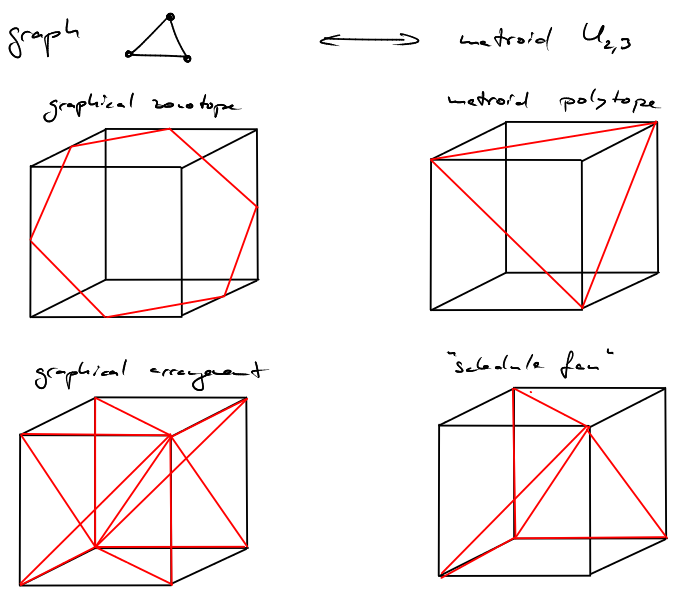
\includegraphics[width=13cm]{graph-matroid}
%% \caption{Difference between graph construction and graphical matroid construction.}
%% \end{figure}


%%
%% ** In Figure 2, we should replace implies with AND to keep everything a Boolean formula over pairwise comparisions. 




\begin{figure}[h]
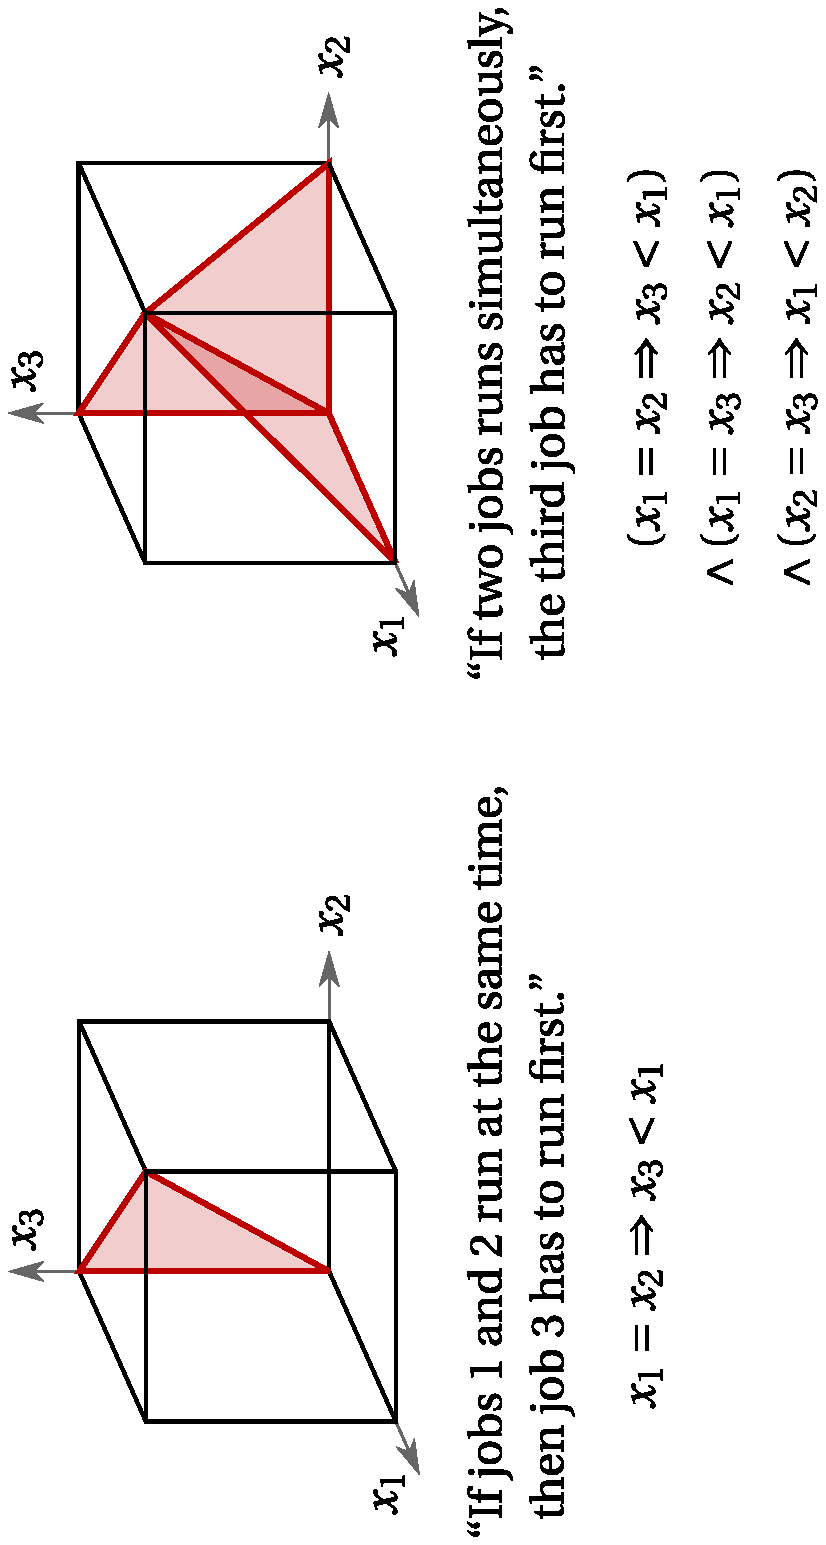
\includegraphics[angle=270,width=4.5in]{schedule}
\label{fig:intro}
\caption{Two scheduling problems and the corresponding geometric configurations. 
  Valid schedules correspond to integer points off of the shaded regions. }
\end{figure}



\section{Preliminaries: Ehrhart Theory}
\label{Ehrhart}

In this section we introduce the basic notions from Ehrhart theory that we need throughout the paper, however we assume some familiarity with polyhedral geometry. As references on these subjects we recommend \cite{Beck2007,Ziegler1995}.

Consider a (bounded) set $X\subset \RR^d$. The \emph{Ehrhart function} 
\[
  \ehr_X:\ZZ_{> 0}\rar\ZZ_{\geq 0}
\]
of $X$ counts the number of integer points in integer dilates of $X$, i.e., 
\[
  \ehr_X(k) = \#\ZZ^d \cap k\cdot X
\]
for any positive integer $k$. Ehrhart's theorem states that if $X$ is a polytope whose vertices have integer coordinates, then the Ehrhart function $\ehr_X$ of $X$ coincides with a polynomial, called the Ehrhart polynomial of the polytope. We call polytopes whose vertices have integer coordinates \emph{integral} or \emph{lattice polytopes}. Two polytopes in $\RR^d$ are \emph{lattice equivalent} if there is an affine automorphism $\phi$ of $\RR^d$ with $\phi(P)=Q$ which induces a bijection on the integer lattice $\ZZ^d$. Lattice equivalent sets $X$ have the same Ehrhart function.

The most important example for our purposes are Ehrhart polynomials of simplices. The $d$-dimensional \emph{standard simplex} $\Delta^d$ is the convex hull of the standard unit vector $e_1,\ldots,e_d\in\RR^{d+1}$, i.e.,
\[
  \Delta^d = \mset{x\in\RR^{d+1}}{\sum_{i=1}^{d+1} x_i =1, x_i \geq 0} 
  = \mset{\sum_{i=1}^{d+1} \lambda_i e_i\in\RR^{d+1}}{\sum_{i=1}^{d+1} \lambda_i = 1, \lambda_i\geq 0, }.
\]
Its Ehrhart polynomial is given by a binomial coefficient
\[
  \ehr_{\Delta^d}(k) = \binom{k+d}{d},
% = \frac{1}{d!} (k+d)\cdot (k+d-1) \cdot \ldots \cdot (k+1)
\]
which is a polynomial of degree $d$ in the variable $k$. An integral simplex is \emph{unimodular} if it is lattice equivalent to a standard simplex, whence all unimodular simplices of the same dimension have the same Ehrhart polynomial. Note that all faces of a unimodular simplex are themselves unimodular simplices.

Ehrhart polynomials of unimodular simplices arise naturally from the study of scheduling problems. Consider the following scheduling problem $S$: ``Schedule two jobs, 1 and 2, such that job 2 starts after or at the same time as job 1." Suppose jobs can be run in $k+1$ discrete time slots, numbered $0$ through $k$. A feasible schedule is a pair of integer numbers $0\leq x_1,x_2 \leq k$ such that $x_1 \leq x_2$. The feasible schedules are precisely the integer points $x=(x_1,x_2)$ contained in the $k$-th dilate of the unimodular simplex $\conv(0,e_2,e_1+e_2)$. Therefore, if we let the deadline $k$ vary, the number of feasible $(k+1)$-schedules is given by the Ehrhart polynomial of a 2-dimensional unimodular simplex, i.e., $\chi_S(k+1)=\ehr_{\Delta^2}(k)=\binom{k+2}{2}$.

If instead, we require job 2 to run strictly after job 1, feasible schedules are then integer points $x\in\ZZ^2$ such that $0\leq x_1,x_2 \leq k$ and $x_1 < x_2$. Denote this scheduling problem by $S'$. The strict inequality gives rise to a \emph{half-open simplex}. The $d$-dimensional standard simplex $\Delta^d_i$ with $i$ open faces is defined just as the standard simplex above, except that $i$ of the inequalities are strict. More precisely
\[
    \Delta^d_i = \mset{x\in\RR^{d+1}}{\sum x_i =1, x_1 \geq 0, \ldots, x_i > 0, x_{i+1} \geq 0, x_{d+1} \geq 0}.
\]
For every face of the standard simplex that we open, the Ehrhart polynomial is shifted by one:
\begin{eqnarray}
  \ehr_{\Delta^d_i}(k) = \binom{k+d-i}{d}.
  \label{eqn:half-open-simplex}
\end{eqnarray}
In particular, the open simplex $\Delta^d_{d+1}$ has Ehrhart polynomial $\ehr_{\Delta^d_{d+1}}(k) = \binom{k-1}{d}$. In the example $S'$, the feasible $(k+1)$-schedules therefore correspond to the integer points in the $k$-th dilate of a $2$-dimensional unimodular simplex with $1$ open face, and their number is $\chi_{S'}(k+1)=\ehr_{\Delta^2_1}(k) = \binom{k+1}{2}$.\footnote{Note that in later sections, we will be using a slightly different setup than in the previous two examples: We will identify time slots with integers $1$ through $k$ by letting $0<x_i<k+1$. This alternate construction then yields $\chi_S(k)=\ehr_{\Delta^2_2}(k+1)=\binom{k+1}{2}$ and $\chi_S(k)=\ehr_{\Delta^2_3}(k+1)=\binom{k}{2}$.}

Half-open simplices do not suffice to capture all scheduling problems. Consider the following example $S''$ of a scheduling problem on three jobs: "Either run all three jobs at the same time, or first job 1, then job 2, and then job 3." A feasible $(k-1)$-schedule is a triple $(x_1,x_2,x_3)$ with $0< x_1,x_2,x_3 < k$ such that $x_1<x_2<x_3$ or $x_1=x_2=x_3$. The resulting geometric region is the union of an open 3-dimensional simplex and (the relative interior of) the main diagonal of the cube $[0,k]^3$. This set is no longer a half-open simplex. In fact, it is not even the set-theoretic difference of two closed polytopes. In order to capture this type of geometric object, we work with partial polytopal complexes.

%

A \emph{polytopal complex} $K$ is a finite set of polytopes in some $\RR^d$ such that $K$ is closed under taking faces and the intersection of any two polytopes in $K$ is a face of both. A polytopal complex is \emph{integral} if all vertices have integer coordinates. We define the \emph{relative interior} $\relint(P)$ of a polytope $P$ to be the interior of the polytope taken with respect to its affine hull, so that, for example, the interior of a 2-dimensional triangle in 3-space is the triangle minus its edges and vertices and, more generally, $\relint{\Delta^d} = \Delta^d_{d+1}$.
 The union of all faces of a polytopal complex is equal to the disjoint union of the relative interiors of all faces. For example, a triangle is equal to the open 2-dimensional region, plus the open line segments corresponding to the edges, plus the vertices (which are open with respect to their 0-dimensional affine hull). This observation implies that the Ehrhart function of a polytopal complex is just the sum of all Ehrhart functions of the relative interiors of all faces.

Now, returning to the example $S''$, the set $X$ of feasible points $x\in\RR^3$ for $k=1$ can be written as the disjoint union of the open 3-dimensional simplex $\sigma$ which is the relative interior of the convex hull of the vectors $(0,0,0)$, $(0,0,1)$, $(0,1,1)$ and $(1,1,1)$ and the open line segment $\lambda$ which is the relative interior of the convex hull of $(0,0,0)$ and $(1,1,1)$. Then the feasible $(k-1)$-schedules are precisely the integer points in $k\cdot X$, i.e., 
\[
\chi_{S''}(k-1)=\ehr_X(k) = \ehr_{\Delta^2_3}(k) + \ehr_{\Delta^1_2}(k) = \binom{k-1}{2} + \binom{k-1}{1}.
\]
However, we note that the triangle $\tau$ that is the relative interior of the convex hull of $(0,0,0)$, $(0,0,1)$ and $(1,1,1)$ is not contained in $X$, even though $\tau$ is a face of $\sigma$ and $\lambda$ is a face of $\tau$. This idea of taking the relative interiors of just some of the faces of a polytopal complex gives rise to the notion of a partial polytopal complex, which was introduced in \cite{fstar}. A \emph{partial polytopal complex} is a subset of the faces of a polytopal complex; in particular, a partial polytopal complex is not closed under taking faces. The \emph{support} $|K|$ of a partial polytopal complex $K$ is the union of the relative interiors of all faces contained in $K$. By abuse of terminology, we will often refer to both $K$ and $|K|$ as the polytopal complex $K$ and let it be clear from context whether we are referring to the subset of Euclidean space or the set of polytopes ordered by the face relation.

Note that in the above example it is still convenient to speak of $(0,0,0)$, $(0,0,1)$, etc.\ as vertices of $\sigma$ and, consequently, as vertices of $X$, even though they are neither contained in $X$ nor in the relative interior of $\sigma$. It will generally be clear from context, whether we are referring to vertices that are actually contained in $X$, or merely to vertices of the closure of some face of the partial complex. However, when we need to carefully distinguish between these two cases, we adopt the following terminology: We call the relative interior of a polytope $P$ an \emph{open polytope}. The \emph{faces of an open polytope} are the faces of its closure. By extension, we define the \emph{closure} of any set of open polytopes as the set of all faces of these polytopes. A \emph{partial polytopal complex} $K$ is now any set of open polytopes whose closure $\bar{K}$ is a polytopal complex. This allows us to distinguish between the faces of a partial polytopal complex $K$ and the faces of its closure $\bar{K}$. Note that indeed $\overline{|K|}=|\bar{K}|$, i.e., the closure of the support is the support of the closure.
%% We will at certain points need to distinguish between the faces of $K$ and the faces of $\bar{K}$. For example, let $K$ be the interior of a triangle together with one of its vertices. In this case, $K$ will have just two faces: the open triangle and the vertex. However, we will have recourse to refer to the other faces of the (closed) triangle as well. These make up the faces of $\bar{K}$.

%The Ehrhart function of a partial polytopal complex is the Ehrhart function of its support. If the complex is integral it is straightforward to show that the Ehrhart function is again a polynomial. In the example of the half-open simplex with the extra point, we can thus observe that its Ehrhart function is $\binom{k+1}{2} + 1$.

%This motivates the following observation: If $K$ is a partial simplicial complex in which all vertices are integral and all simplices are unimodular. Then, the Ehrhart function $\ehr_K$ satisfies
%\[
%  \ehr_K(k) = \sum_{i=0}^d f_i^* \binom{k-1}{i}
%\]
%where $d$ is the dimension of $K$ and $f_i^*$ denotes the number of $i$-dimensional faces in $K$.  The polynomials $\binom{k+d-i}{d}$ form a basis of the space of polynomials of degree at most $d$. Thus every Ehrhart polynomial can be written in the above form and the $f_i^*$ are the coefficients of the polynomial with respect to this binomial basis. Intuitively, the coefficients $f_i^*$ count how many unimodular simplices of dimension $i$ the complex contains. This will be made precise in Section~\ref{sec:scheduling-problems}.

\section{Preliminaries: Coxeter Complexes, QSym and NCQsym}
\label{ncqsym}


Suppose we are given a scheduling problem with $3$ jobs and three types
of constraints. Any of the three jobs may be started first but different
requirements are imposed depending on which starts first.  If jobs $1$ or $3$ are started first, then the other must start at the same time.  If job $2$ starts first, then job $1$ must occur next before job $3$ can be started: 
\begin{align*}
(x_1 < x_2) &\wedge (x_2 = x_3)\\
(x_3 < x_2) &\wedge (x_1 = x_2)\\
(x_2 < x_1) &\wedge (x_1 < x_3).
\end{align*}
We can interpret the solutions as all those integer points such that
$x_1 < x_2 = x_3$ or $x_3 < x_1 = x_2$ or $x_2 < x_1 < x_3$.
Importantly, solutions only depend on the relative ordering of
coordinates.  It is this observation that allows solutions to be
indexed by ordered set partitions.



An \emph{ordered set partition} or \emph{set composition} $\Phi \vDash
[n]$ is a sequence of sets $(\Phi_1, \Phi_2, \ldots, \Phi_k)$ such
that for all $i,j$, ($ \Phi_i \cap \Phi_j = \emptyset$) and
($\cup_i \Phi_i = [n]$).  The $\Phi_i$ are the blocks of the ordered
set partition and we will often use the notation $\Phi_1| \Phi_2|
\cdots| \Phi_k$.  Note that within each block, elements are not
ordered, so the ordered set partition $13|4|2 \vDash [4]$ is the same
as $31|4|2 \vDash [4]$.  We will use ordered set partitions to represent integer
points whose relative ordering of coordinates is given by the blocks
of the partition.  For example, $31|4|2$ represents all integer points
such that $x_1 = x_3 < x_4 < x_2$.  As solutions to scheduling
problems are naturally indexed by ordered set partitions they are
closely related to the algebra of quasisymmetric functions in
non-commuting variables, NCQSym, and the Coxeter complex of type $A$,
$\cox_A$. In particular, the scheduling polynomial counts the number
of solutions to a scheduling problem.  We will interpret this
polynomial as a specialization of the NCQSym scheduling function.

\subsection{The Coxeter Complex of Type A}
The braid arrangement $\mathcal{B}_n$ is the hyperplane arrangement in
$\mathbb{R}^n$ consisting of hyperplanes $x_i = x_j$ for all $i,j \in [n]$.
This arrangement is central, that is all hyperplanes contain
the origin.  It is also non-essential, that is the collection of
normals to the hyperplanes do not span all of $\mathbb{R}^n$.  The
hyperplanes have a common intersection equal to the line $x_1 = x_2 = \cdots
= x_n$.  Projecting the arrangement to the orthogonal complement of
this line and intersecting with the unit sphere yields a spherical
simplicial complex known as the \emph{Coxeter complex of type $A$}, $\cox_A$.
It can be realized combinatorially as the baricentric subdivision of the
boundary of the simplex.  In the Erhart setting of the previous section, this complex
can be obtained by (1) starting with the cube $[0,1]^d$, (2) triangulating 
this with the braid arrangement, and (3) removing the two vertices consisting of 
only zeros and only ones, and all incident faces. 

%** fb: Also, should we mention here that the Coxeter complex is the dual of the face lattice of the permutahedron? **

The faces of $\cox_A$ are naturally  labeled by ordered
set partitions.  Each face of the Coxeter complex is simply a
normalization of a face of the cell decomposition induced by
$\mathcal{B}_n$ on $\mathbb{R}^n$.  A face of the cell decomposition of $\mathcal{B}_n$ specifies for each pair $i,j$ whether $x_i < x_j$, $x_i > x_j$, or $x_i = x_j$, precisely the atomic formulas of scheduling problems.  All points in a fixed face have
the same relative ordering of coordinates.  This relative ordering
induces an ordered set partition on $[n]$.  For example, if a face
consists of all points such that $x_2 = x_3 < x_1 =
x_4 = x_6 < x_5$ then the induced ordered set partition is
$23|146|5$.  Under this correspondence, we see that each maximal face
corresponds to a partition into blocks of size one (i.e. a full
permutation).  Moreover, a face $F$ is contained in a face $G$ if and only if
the ordered set partition corresponding to $F$ coarsens the ordered set partition
corresponding to $G$; the face lattice is dual to the face lattice of the permutahedron.
%  Hence a collection of ordered set partitions closed under coarsening gives a subcomplex of the Coxeter complex.

\begin{figure}[h]
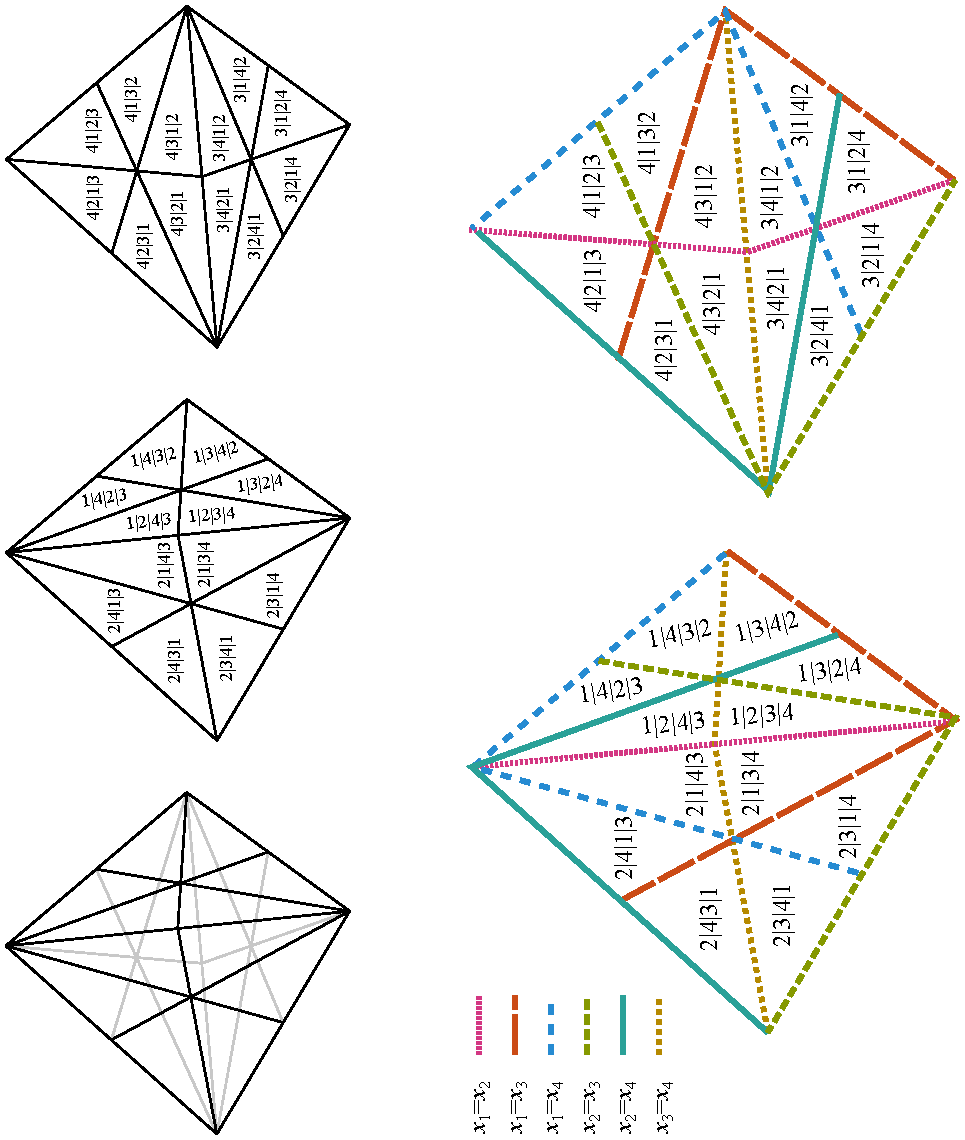
\includegraphics[angle=270,width=5.5in]{coxeter.pdf}
\caption{Top row: The Coxeter complex of type A on $4$ elements. Left image shows entire complex realized as barycentric subdivision of the boundary complex of a tetrahedron. The two images to the right show front and back faces labeled by ordered set partitions. Bottom row: The front and back faces of the Coxeter complex with edges marked to show corresponding hyperplanes of braid arrangement.}
\end{figure}

\subsection{NCQSym}


Let $\{x_1, x_2, \ldots \}$ be a collection of non-commuting
variables.  Given $a \in \mathbb{N}^n$, let $\Delta(a)$
be the ordered set partition $(\Delta_1 | \Delta_2 | \ldots | \Delta_k)$ such that 
%flag of subsets $\empty = F_0 \subset F_1 \subset \ldots
%\F_{k+1} =[n]$ such that 
$a$ is constant on each set $\Delta_i$
%\backslash F_{i-1}$ 
and satisfies $a|_{\Delta_i} < a|_{\Delta_{i+1}}$ for all $1 \leq i \leq k$. 
%We call $\mathcal{F}(\omega)$ the flag of $\omega$ and
Define the \emph{order class} of $a$ to be the set of vectors $b$
such that $\Delta(b) = \Delta(a)$.  
%The order class of $a$ consists of all 
%points such that the relative size of their components is the same.  If $a$ is contained in the relative interior of the face $F$ of the Coxeter complex, then the order class of $a$ consists of all integer points in the relative interior of $F$.

\begin{example}
For $a = (3,2,2,3,1) \in \mathbb{N}^5$, $\Delta(a) =
(5|23|14)$.  The order class of $a$ consists of all vectors $x
\in \mathbb{N}^5$ such that $x_5 < x_2 = x_3 < x_1 = x_4$. 
\end{example}


The order class specifies the relative ordering of coordinates and contains all points in the relative interior of a cone
of the braid arrangement.  Hence an order class is naturally associated to (the relative interior) of a face of
the Coxeter complex.  
The solutions to a satisfiable scheduling problem correspond to a union of these open faces.   


\begin{definition}
A function in non-commuting variables is called quasisymmetric (an element of NCQSym) if
$\forall \, \gamma, \tau \in \mathbb{N}^n$ such that $\gamma$ and $\tau$
are in the same order class, $\Delta(\gamma) =
\Delta(\tau)$, the coefficient of $x_{\gamma_1}x_{\gamma_2} \cdots
x_{\gamma_n}$ is the same as the coefficient of $x_{\tau_1}x_{\tau_2} \cdots x_{\tau_n}$.
\end{definition}

Let $\Phi$ be an ordered set partition.  Define the monomial quasisymmetric function in non-commuting variables indexed by $\Phi$ as follows:
$$\ncM_{\Phi} = \sum_{a \in \mathbb{N}^n \, \Delta(a) = \Phi} {\bf{x}}_{a}.$$

Alternatively, quasisymmetric functions in non-commuting variables can be defined as any function which can be expressed as a sum of monomial terms $\ncM_{\Phi}$.

\begin{example}
Consider the order class of points that satisfy $x_1 = x_3 < x_2 =
x_4$.  The corresponding ordered set partition $\Phi$ is $(13|24)$.
$$\ncM_{13|24} = x_1x_2x_1x_2 + x_1x_3x_1x_3 + x_2x_3x_2x_3 + x_3x_4x_3x_4 + \cdots$$  
\end{example}



 One of the staples of geometric methods in combinatorics is to
 interpret a monomial as an integer point in space. The standard
 construction is to view a monomial in commuting variables
 $x_1^{a_1}x_2^{a_2}\cdot\ldots\cdot x_d^{a_d}$ as the point
 $(a_1,a_2,\ldots,a_d)\in\ZZ^d$. To translate quasisymmetric functions
 in non-commuting variables into a geometric setting, we need to use a
 different construction. Here we associate to a monomial
 $x_{i_1} x_{i_2} \cdot \ldots \cdot x_{i_d}$ the point
 $(i_1,\ldots,i_d)\in \ZZ^d$. For example $x_2x_1x_3$ becomes
 $(2,1,3)\in\ZZ^3$. That is, the entries of the vector are given by
 the \emph{indices} of the monomial, as opposed to the exponents. This
 is well defined because we are working with non-commuting variables, so
  the factors $x_i$ appear in a fixed order.

Figure~\ref{fig:cone} provides examples of this construction.  When viewed
through the geometric lens explained above the infinite formal sum
$\sum_{0<i_3<i_1<i_2} x_{i_1}x_{i_2}x_{i_3}$ in the non-commuting
variables $\{x_1,x_2,x_3,\ldots\}$, corresponds to the set of integer
points $z\in\ZZ^3$ with $0<z_3<z_1<z_2$, that is, the set of integer
points in the relative interior of the cone generated by vectors
$e_2,e_1+e_2$ and $e_1+e_2+e_3$. If we turn one of the two
inequalities into equalities, i.e., we pass to the sums
$\sum_{0<i_3<i_1 = i_2} x_{i_1}x_{i_2}x_{i_3}$ and
$\sum_{0<i_3=i_1<i_2} x_{i_1}x_{i_2}x_{i_3}$, we obtain two facets of
this cone. More precisely, we obtain the set of lattice points in the
relative interiors of the cones $\cone_\ZZ(e_1+e_2,e_1+e_2+e_3)$ and
$\cone_\ZZ(e_2,e_1+e_2+e_3)$, respectively.


\begin{figure}[h]
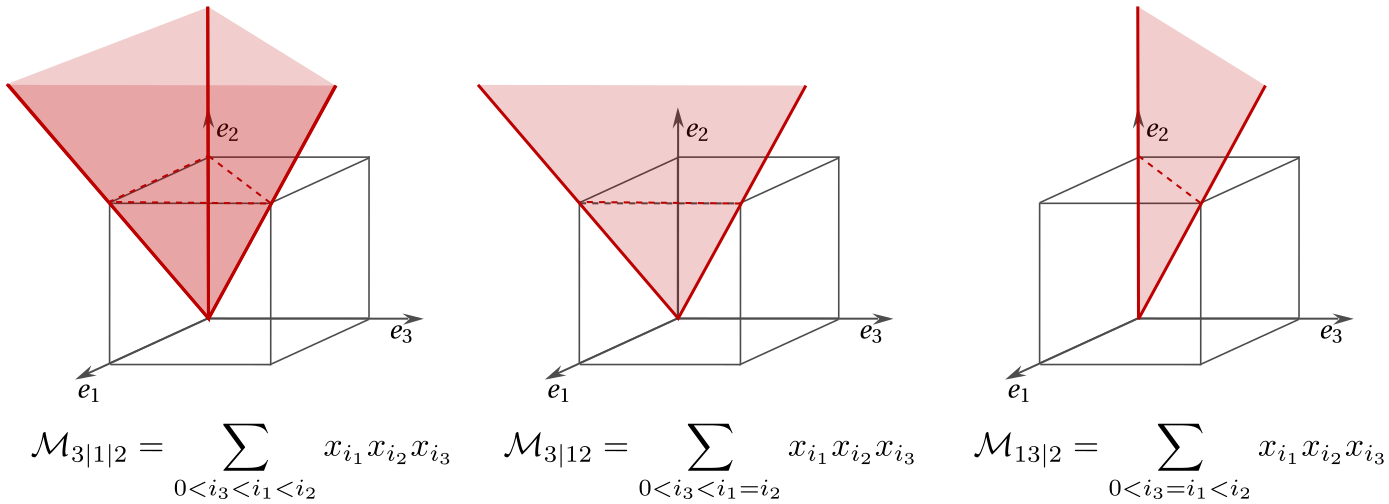
\includegraphics[angle=270,width=14cm]{cone}
\caption{\label{fig:cone}Correspondence between monomial nc-quasisymmetric functions and simplicial unimodular cones in the braid arrangement.}
\end{figure}



We will sometimes refer to quasisymmetric functions in non-commuting
variables as nc-quasisymmetric functions.  Informally, an
nc-quasisymmetric function corresponds to a $k$-schedule where $k$ has
been taken to infinity, i.e. there is no deadline.  Recall the example
above on two jobs such that job 2 must start after job 1 unless they
start at the same time.  The solutions corresponds to the integer points satisying $\{x_1 < x_2\}$ or $\{x_1 = x_2\}$ and are recorded by the
nc-quasisymmetric function $\ncM_{1|2} + \ncM_{12}$.

\begin{definition}
Given a scheduling problem $S$, the scheduling quasisymmetric function in noncommuting variables is the sum of monomial quasisymmetric functions in non-commuting variables $\ncM_{\Phi}$ over all ordered set partitions ${\Phi}$ such that $S$ is satisfied by any (and hence all) integer points $a \in \mathbb{N}^k$ with relative ordering given by $\Phi$,

$$ \ncS_S = \sum_{\substack{\Phi, \, \Delta(a) =\Phi \\ a \, {\operatorname{satisfies}} \,S}} \ncM_{\Phi}. $$

\end{definition}





\subsection{From NCQsym to QSym to Polynomials}


 In order to impose a deadline, or $k$ time slots, we restrict to
 a finite number of non-zero variables.
Although not strictly necessary to arrive at a polynomial, we will also be interested in the intermediate specialization from an nc-quasisymmetric function to a quasisymmetric function.  


A \emph{quasisymmetric function} is a formal power series in infinitely many
variables $\{x_1, x_2, \ldots \}$ which has bounded degree and is shift invariant.  Namely, for
any composition $\alpha$, the coefficients of all terms,
$x_{i_1}^{\alpha_1}x_{i_2}^{\alpha_2} \cdots x_{i_k}^{\alpha_k}$,
running over all possible $k$-tuples, $\{i_1 < i_2 < \ldots < i_k \}$, are
the same.


The monomial quasisymmetric function indexed by the composition $\alpha$ is 
$$M_{\alpha} := \sum_{1 \leq i_1 < i_2 < \ldots < i_k}
x_{i_1}^{\alpha_1} \ldots x_{i_k}^{\alpha_k}.$$  One may equivalently
define quasisymmetric functions as any series which can be written as a
linear combination of monomial quasisymmetric functions.



Thus elements of QSym are naturally indexed by
compositions and elements of NCQSym are naturally indexed by ordered
set partitions.  
The \emph{type map} maps elements of NCQSym to Qsym by sending ordered set partitions to compositions.
 %We can use the type map from partitions to
%compositions to specialize an element of NCQSym to an element of QSym.
The type map of an ordered set partition simply records the size of each block:
$$\type(\Phi_1|\Phi_2|\cdots|\Phi_n) = (|\Phi_1|, |\Phi_2|, \cdots, |\Phi_n|).$$
If $\mathcal{S} \in$ NCQSym is written as a sum of monomial terms,
applying the type map to each index is equivalent to allowing the
variables to commute.  In this way we extend the type map to nc-quasisymmetric functions themselves.

\begin{example}
Let $$\mathcal{F} = \ncM_{1|23} + \ncM_{3|21} + \ncM_{2|1|3}$$ be an element of NCQSym written in terms of monomials.  Then 
\begin{align*}
\textrm{type}(\mathcal{F}) & =  M_{\textrm{type} (1|23)} + M_{\textrm{type} (3|12)} + M_{\textrm{type} (2|1|3)} \\
&  = 2 M_{(1,2)} + M_{(1,1,1)} \in \textrm{QSym}.
\end{align*}
\end{example}



Given a quasisymmetric function in non-commuting variables (or
commuting), there is a naturally associated polynomial function
defined by setting the first $k$ variables $x_1, x_2, \ldots, x_k$ equal to $1$. For a single monomial term we have
$$\ncM_{\Phi} ({\bf 1}^k) = { k \choose \ell(\Phi) },$$
where $\ell(\Phi)$ is equal to the length, i.e. the number of blocks, of the partition.

%%  For a scheduling problem, this polynomial counts the number of $k$-schedules.
%% In general, the schedule counting polynomial $\poly_S(k)$ is defined as
%% \[
%%   \poly_S(k) = \# \text{$k$-schedules $\omega$ such that $\phi(\omega)$ is true}.
%% \]
%%  As we will solidify in the next section,  for a scheduling problem $S$, 
%% \[
%%   \SSS_S({\bf 1}^k) = \poly_S(k).
%% \]

\begin{example}
 Continuing the example above gives
$$\mathcal{F} = \ncM_{1|23} + \ncM_{3|21} + \ncM_{2|1|3}$$
$$ \mathcal{F}({\bf 1}^k) = 2 {k \choose 2} + {k \choose 3}.$$  
\end{example}

%% In summary, we have the following lemma.

%% \begin{lemma}
%% If $S$ is a scheduling problem on $n$ items, then $\SSS_S$ is an ncquasisymmetric function and $\poly_S$ is a polynomial of degree at most $n$. Moreover, $\SSS_S$ specializes to $\poly_S(k)$ when we substitute $1$ for $k$ different variables in $\SSS_S$ and $0$ for all others, i.e.,
%% \[
%%   \SSS_S({\bf 1}^k) = \poly_S(k).
%% \]
%% Note that the result of this specialization is independent of which variables are set to 1.
%% \end{lemma}

%% \comment{fb: We should add a statement about quasisymmetric functions to this lemma.}



\section{Scheduling Problems}
\label{sec:scheduling-problems}

In this section we bring the varying perspectives of Ehrhart theory, Coxeter complexes and quasisymmetric functions together to prove basic properties of scheduling problems.  First, for any scheduling problem $S$, the number of $k$-schedules satisfying $S$ is seen to be a polynomial function in $k$.  This scheduling polynomial is both an Ehrhart polynomial and a polynomial specialization of a quasisymmetric function.  Next,we define the allowed and forbidden scheduling subconfigurations and connect the geometry of these spaces to the scheduling polynomial.  Specifically, it is shown that the $h$-vectors of (shifted) scheduling polynomials are equal to the the $h$-vectors of the allowed and forbidden subconfigurations.  


\begin{definition}
A \defn{scheduling problem} on $d$ items is given by a boolean
formula $S$ over atomic formulas $\omega_i\leq \omega_j$ for
$i,j\in[d]$. A \defn{$k$-schedule} solving $S$ is a function
$\omega:[d]\rightarrow[k]$ such that $S(\omega)$ is true.
\end{definition}



For an ordered set partition $\Phi=(\Phi_1,\ldots,\Phi_m)$, we define the relatively open cone $\cone(\Phi)\subset\RR^n$ to be the set of all $a\in\RR^n$ that satisfy the constraints
\begin{eqnarray*}
0 < a_i && \text{for all $i\in[n]$}, \\
a_i = a_j && \text{for all $l\in[m]$ and $i,j\in\Phi_l$}, \\
a_i < a_j && \text{for all $l_1 < l_2\in[m]$ and all $i\in\Phi_{l_1}, j\in\Phi_{l_2}$}.
\end{eqnarray*}
Equivalently, $\cone(\Phi)$ is the set of all real vectors $a$ in the positive orthand, $\RR_{> 0}^n$ such that $\Delta(a)=\Phi$: 
\[
\cone(\Phi) = \mset{a\in\RR_{> 0}^n}{\Delta(a)=\Phi}.
\]
 If $\Phi$ ranges over all ordered set partitions of $[n]$, these cones form a triangulation $T^n$ of the positive orthand $\RR_{> 0}^n$, 
\[
  \RR_{> 0}^n = \bigcup_\Phi \cone(\Phi).
\]


This triangulation of $\RR_{> 0}^n$ can also be obtained by subdividing the positive orthand according to the braid arrangement of all hyperplanes $x_i=x_j$. Combinatorially, the resulting partial polyhedral complex is equivalent to a cone over the Coxeter complex of type $A$. 

As discussed in the previous section, we associate to every $a\in\NN^n$ a monomial in non-commuting variables $x_{a_1}\cdots x_{a_n}$ which we abbreviate as ${\bf x}_a$. In this way, we can associate to every set of lattice points, $A\subset\NN^n$, a formal sum $N(A)$ of monomials in non-commuting variables
\[
  N(A) = \sum_{a\in A} {\bf x}_a.
\]

The function $N$ maps $\cone(\Phi)$ to the monomial nc-quasisymmetric functions $\ncM_\Phi$,
\[
  N(\cone(\Phi)\cap\ZZ^n) = \ncM_\Phi.
\]
Conversely, we can think of any nc-quasisymmetric function $\mathcal{F}$ with non-negative coefficients in the monomial basis as a multiset of cones in the positive orthand, where the multiplicity of lattice points in $\cone(\Phi)$ is given by the coefficient of $\ncM_\Phi$ in $\mathcal{F}$.
%\comment{Refer back to an example or make an example}
% In the case of scheduling ncquasisymmetric functions we can conclude that for any scheduling problem $S$, the ncquasisymmetric function $\SSS_S$ has coefficients $0$ or $1$ in the monomial basis.



%As we will see below, $\cone(\Phi)\cap(0,1)^n$ is a relatively open unimodular simplex of dimension $m$, hence
%\[
 % \poly_\Phi(k) = \binom{k}{m}.
%\]



Let $S$ be a scheduling problem on $n$ items. For any vector $a\in\RR^n_{> 0}$ we write $S(a)$ to denote the boolean value of whether or not $a$ satisfies the constraints imposed by $S$.  $S(a)$ depends only on the relative order of the components $a_i$, and therefore is entirely determined by the ordered set partition $\Phi=\Delta(a)$. We use $S(\Phi)$ to denote the boolean value of whether or not $S(a)$ is satisfied for any (or, equivalently, all) $a$ with $\Delta(a)=\Phi$. Geometrically, this means that $S$, viewed as a function on $\RR^n_{>0}$, is constant on each of the open cones, i.e., on the relative interior of, each face of the above triangulation $T^n$ of $\RR^n_{> 0}$.

These observations lead to the following theorem about scheduling counting functions. 

%coefficients of the generating functions $\SSS_S$ in the monomial basis and the coefficients of the scheduling function $\poly_S$ in the binomial basis.


\begin{theorem}
\label{fbasis}
Let $S$ be a scheduling problem on $n$ items.
%%  and $\SSS_S$ the nc-quasisymmetric function of the form
%% \[
%%   \SSS_S = \sum_{\Phi:S(\Phi)} \ncM_\Phi
%% \]
%% where the sum ranges over all ordered set partition $\Phi$ that satisfy $S$. 
%% %In particular, the coefficients of $\SSS_S$ in the monomial basis are either 0 or 1.
% $\poly_S$,
The scheduling counting function,
 $$\poly_S(k) = \textrm{ the number of $k$-schedules satisfying $S$}, $$ is a polynomial in $k$.
  Its degree is at most $n$ and the coefficients $f_1,\ldots,f_n$ of $\poly_S$, given by
\[
  \poly_S(k) = \sum_{i=1}^n f_i\binom{k}{i}
\]
%or, equivalently,
%\[
%  z^{-1}\sum_{k\geq 1} \ehr_S(k)z^k = z^{-1}(\frac{f_0z^1}{(1-z)^1} + \cdots + \frac{f_dz^{d+1}}{(1-z)^{d+1}})
%  z^{-1}\sum_{k\geq 0} \ehr_S(k+1)z^{k+1} = ...
%  \sum_{k\geq 0} \ehr_S(k+1)z^k = ...
%\]
%\[
%  \sum_{k\geq 0} \poly_S(k)z^k = \frac{f_1z^1}{(1-z)^2} + \cdots + \frac{f_nz^{n}}{(1-z)^{n+1}},
%\]
are positive integers bounded above by $i!\cdot S(n,i)$. where the $S(n,i)$ are the Stirling numbers of the second kind.


%% satisfy the following properties:
%% \begin{enumerate}
%% \item $f_i\in\ZZ$,
%% \item $0\leq f_i \leq ,
%% \item $f_i$ counts the number of ordered set partitions $\Phi$ of $[n]$ into $i$ non-empty parts such that $S(\Phi)$ holds.
%% \end{enumerate}
\end{theorem}

\begin{proof}
Let $S$ be a scheduling problem. Let $A$ denote the set of all vectors $a\in\RR^n_{> 0}$ such that $S(a)$ holds true. Recall that the scheduling nc-quasisymmetric function is
\[
 \SSS_S = \sum_{a\in A\cap\ZZ^n} {\bf{x}}_a = \sum_{\Phi:S(\Phi)} \ncM_\Phi,
\]
where the latter sum ranges over all ordered set partitions $\Phi$ for which $S(\Phi)$ holds true. This means in particular that the coefficients of $\SSS_S$ in the monomial basis are either 1 or 0, indicating which open cones $\cone(\Phi)$ are contained in $A$ and which are disjoint from $A$.

Let $\Phi$ be an ordered set partition with $n$ non-empty parts, i.e., a permutation of the numbers $1,\ldots,n$. Assume without loss of generality that $\Phi=1|2|\cdots|n$. Then
\[
  \cone(\Phi)\cap [0,1]^n = \mset{a\in[0,1]^n}{a_1<a_2<\ldots<a_n}
\]
which is easily seen to be a unimodular simplex with vertices $(0,\ldots,0)$, $(0,\ldots,0,1)$, $(0,\ldots,0,1,1)$, $\ldots$, $(1,\ldots,1)$. If, more generally, $\Phi=(\Phi_1,\ldots,\Phi_i)$ is any ordered partition with $i\in[n]$ non-empty parts, then $\cone(\Phi)\cap[0,1]^n$ is an $i$-dimensional unimodular simplex with vertices $v_0,\ldots,v_i$ where $v_j$ for $j=0,\ldots,i$ has entries 
\[
 v_{j,k} = \choice{1 & \text{if }k\in\Phi_{i-l} \text{ for some } 0\leq l < j, \\ 0 & \text{otherwise.} }
\]
In particular, $v_0= \mathbf{0}$ and $v_i=\mathbf{1}$. 

Passing to the open cube, we find that the collection of relatively open simplices $\cone(\Phi)\cap (0,1)^n$ where $\Phi$ ranges over the ordered set partitions of $[n]$ is a partial simplicial complex that triangulates the open cube $(0,1)^n$. If $\Phi$ has $i$ parts, then $\cone(\Phi)\cap (0,1)^n$ is a relatively open $i$-dimensional simplex whose Ehrhart polynomial is
\[
  \ehr_{\cone(\Phi)\cap (0,1)^n}(k) = \binom{k-1}{i} = \#\cone(\Phi)\cap (0,k)^n \cap \ZZ^n.
\] 


Given a nc-quasisymmetric function, substituting 1s for variables $x_1,\ldots,x_k$ and $0$s for variables $x_{k+1},\ldots$  sets all monomials ${\bf x}_a$ to $1$ for which $a_i \leq k$ for all $i$, and all monomials ${\bf x}_a$ to $0$ for which $a_i > k$ for some $i$. Thus substituting ${\bf 1}^k$ into $\ncM_\Phi$ corresponds to taking the intersection of $\cone(\Phi)$ with the open cube $(0,k+1)^n$, i.e.,
\[
 N(\cone(\Phi)\cap(0,k+1)^n\cap\ZZ^n) = \ncM_\Phi({\bf 1}^k).
% =  \poly_\Phi(k). 
\]
We observe that
\[
  \cone(\Phi)\cap(0,k+1)^n = (k+1)\cdot (\cone(\Phi)\cap(0,1)^n), 
\]
since the hyperplanes defining $\cone(\Phi)$ all go through the origin. We have thus found that
\begin{eqnarray}
\label{eqn:spec ncM}
  \ncM_\Phi({\bf 1}^k) 
%= \poly_\Phi(k) 
= \ehr_{\cone(\Phi)\cap(0,1)^n}(k+1),
\end{eqnarray}
that is, $\ncM_\Phi({\bf 1}^k)$ is the Ehrhart polynomial of the open polytope $\cone(\Phi)\cap(0,1)^n$, up to a shift of 1. 





It follows that
\begin{eqnarray*}
  \poly_S(k) &=& \#A\cap(0,k+1)^n\cap\ZZ^n \\
  &=& \ehr_{A\cap(0,1)^n}(k+1) \\
  &=& \sum_{\Phi:S(\Phi)} \ehr_{\cone(\Phi)\cap(0,1)^n}(k+1) \\
  &=& \ncM_{\Phi}({\bf 1}^k) \\  
&=& \sum_{i=1}^n f_i\binom{k}{i}
\end{eqnarray*}
where $f_i$ is the number of ordered set partitions $\Phi$ with $i$ non-empty parts. Note that the binomial coefficients $\binom{k}{i}$ for $i=0,\ldots,n$ form a basis of the space of polynomials of degree at most $n$, so the coefficients $f_i$ are determined by the polynomial $\poly_S(k)$. 
%To see that the above generating function definition of the coefficients $f_i$ is equivalent, note that 
%\[
%  \frac{1}{(1-z)^{d+1}} = \sum_{k\geq 0} \binom{k+d}{d} z^k
%\]
%from which we get the desired identity by algebraic manipulation.

From this counting interpretation of the coefficients $f_i$ it follows immediately that the $f_i$ are non-negative integers. Moreover there are at most $i!\cdot S(n,i)$ ordered set partitions of $[n]$ with $i$ non-empty parts, which proves the upper bound on the $f_i$. 

%Finally, the fact that $\SSS_S$ specializes to $\poly_S(k)$ follows immediately from the specialization (\ref{eqn:spec ncM}).
\end{proof}


\begin{example}
In our running example of two jobs in which job $1$ may start before job $2$ or both jobs can start simultaneouly but job $2$ can not start before job $1$, the nc-quasisymmetric scheduling funciton was $\ncM_{1|2} + \ncM_{12}$.  Thus the scheduling polynomial is
$$\poly_S(k) = \SSS_S({\bf 1}^k) = \binom{k}{2} + \binom{k}{1}.$$
\end{example}



\begin{example}
A particularly familiar example of a scheduling problem is graph
coloring.  Given a finite graph $G = (V,E)$, a $k$-coloring of $G$ is
an assignment $\phi(G): V \rightarrow [k]$ such that for all edges
$\{i,j\} \in E$, $\phi(v_i) \neq \phi(v_j)$.  Namely, a
$k$-coloring colors the vertices of a graph with at most $k$-colors
such that if two vertices are joined by an edge, then they are given
different colors.  As a scheduling problem, the edges of the graph
give strict atomic formulas: for all edges $\{i,j\} \in E$, $x_i
\neq x_j$.  

The scheduling quasisymmetric functions are in fact symmetric in the
chromatic case.  The chromatic symmetric function in non-commuting
variables was introduced by Gebhard and Sagan~\cite{GS} and the
chromatic symmetric function was introduced by
Stanley~\cite{stan-chromatic}.  The scheduling counting function is
the well studied chromatic polynomial.  We point out that the
chromatic counting function is usually established to be a polynomial
using a contraction deletion argument on the edges of a graph.  Our
method instead establishes this function as a polynomial via a
specialization of a symmetric function and as an Ehrhart polynomial.  We will recover much of the well-known structure of these functions by considering the geometry of the scheduling solutions, as seen in the next section.

%% Chromatic - discuss Chromatic as Scheduling problem, ncsym, sym, polynomial. Establishes polynomiality without contraction deletion.  $\poly_S$ is the chromatic polynomial.  The quasisymmetric function obtained by taking the type map on $\SSS_S$ is Stanley's chromatic symmetric function (the quasisymmetric function happens to be fully symmetric in this case).  Gebhard and Sagan studied (essentially) $\SSS_S$ as a symmetric function in non-commuting variables.
\end{example}


\subsection{Triangulations and their Allowed and Forbidden configurations}
\label{sec:allow-forb-configurations}
Geometrically we have seen that
the braid arrangement, consisting of all hyperplanes
\[
  H_{i,j} = \mset{a\in\RR^n}{a_i = a_j}
\]
for $1\leq i,j\leq n$, induces subdivisions $\TRn$, $\TP$, $\TC$, and $\TS$ of the space $\RR^n$, the positive orthand $\RR^n_{> 0}$, the open unit cube $(0,1)^n$ and the $n-2$ dimensional sphere
\[
S^{n-2}=\mset{x\in\RR^n}{||x||_2 = 1, \sum_{i=1}^n = 0}.
\]
 The faces of these subdivisions are the regions of the respective ground set where the function $\Delta$, mapping points $a\in\RR^n$ to ordered set partitions $\Phi$, is constant. The faces of $\TRn$ are relatively open polyhedral cones, each containing the lineality space $\mset{a\in\RR^n}{a_i=a_j \; \forall i,j}$. The faces of $\TP$ are pointed, relatively open simplicial cones. The faces of $\TC$ are relatively open unimodular simplices. The faces of $\TS$ are sections of the $n-2$ sphere. Combinatorially $\TS$ is equivalent to the simplicial complex known as the Coxeter complex of type $A_{n-1}$.

All of these complexes are closely related. In fact, $\TRn$, $\TP$, and $\TC$ are all combinatorially equivalent, as the function $\Delta$ defines a bijection between their sets of faces that preserves incidences. In particular, the faces of these three complexes are in one-to-one correspondence with the ordered set partions $\Phi$ of $[n]$ into non-empty parts. The only difference with $\TS$ is that there is no face of $\TS$ corresponding to the partition with only one part. Combinatorially, the other complexes are the cone over $\TS$. As these geometric objects are so closely related, we will frequently draw no clear distinction between them and refer loosely to the triangulation $\Tn$. It will be clear from context which of these objects we are referring to in each case.

We write $\sigma\in\Tn$ to denote that $\sigma$ is a face of the triangulation $\Tn$. We use $\sigma_\Phi$ to mean the face of $\Tn$ corresponding to the ordered set partition $\Phi$.  Recall that for a scheduling problem $S$, $S(\Phi)$ denotes the truth value of whether $S(a)$ holds for any (or, equivalently, all) $a\in\RR^n$ with $\Delta(a)=\Phi$. We define the \emph{allowed configuration} $\allow(S)$ of the triangulation $\Tn$ to be the set of faces 
\[
  \allow(S) = \mset{\sigma_\Phi \in \Tn}{S(\Phi) \textrm{ holds}}.
\]
Correspondingly, define the \emph{forbidden configuration} $\forb(S)$ to be the set of faces
\[
  \forb(S) = \mset{\sigma_\Phi \in \Tn}{\neg S(\Phi) \textrm{ holds}}.
\]



\begin{example} As remarked above, a particularly familiar scheduling polynomial is the chromatic polynomial of a graph.  In this case, the scheduling problem simply specifies which variables can not be equal to each other, $x_i \neq x_j$ for $\{i,j\}$ an edge of the graph.   Steingrimmson's coloring complex~\cite{Ein} can be described as
the collection of ordered set partitions with at least one edge in at least one block, namely 
the forbidden configuration of the chromatic scheduling problem.  
Much work has been done to understand the coloring complex in particular to better understand the chromatic polynomial.  This avenue is possible because of the Hilbert series connection as shown in~\cite{Ein}.  As we will see below this connection holds more generally for all scheduling problems.
\end{example}

Clearly, $\allow(\neg S)=\forb(S)$. This translates into basic observations about the counting function defined by $S$. Let 
\[
  \SSS_{\NN^n} = \sum_{a\in\NN^n} {\bf x}_a
\]
denote the nc-quasisymmetric function corresponding to all lattice points in the positive orthand. Furthermore, note that $(k-1)^n$ is the Ehrhart polynomial of the open cube $(0,k+1)^n$. 

\begin{lemma}
Let $S$ be a scheduling problem on $n$ items. Let $\neg S$ denote the scheduling problem given by the negative of the boolean fomula $S$. Then 
\begin{eqnarray*}
  \poly_{S}(k) + \poly_{\neg S}(k) &=& (k-1)^n, \\
  \SSS_S + \SSS_{\neg S} &=& \SSS_{\NN^n}.
\end{eqnarray*}
\end{lemma}

%% Note that passing from $\SSS_S$ to $\SSS_{\neg S}$ swaps coefficients 0 and 1 in the monomial basis. Also passing from $\poly_S$ to $\poly_{\neq S}$ replaces the coefficient $f_i$ with $i!\cdot S(n,i) - f_i$, thus interchanging the roles of the upper and lower bound on the $f_i$ in the theorem.

\begin{proof}
The result on $\SSS_S$ is immediate from the above observations. For the result on $\poly_S$, note that 
\[
 \poly_{S}(k) + \poly_{\neg S}(k) = \ehr_{A\cap(0,1)^n}(k+1) +  \ehr_{(0,1)^n\setminus A}(k+1) = \ehr_{(0,1)^n}(k+1) = (k-1)^n.
\]
\end{proof}

We have seen in the preliminaries that the Ehrhart polynomial of a $d$-dimensional unimodular simplex $\Delta^d_i$ with $i$ open faces is
\[
  \ehr_{\Delta^d_i}(k) = \binom{k+d-i}{d}.
\]
A $d$-dimensional simplex can have between 0 and $d+1$ open faces, and the polynomials $\binom{k+d-i}{d}$ for $i=0,\ldots,d+1$ generate the space of all polynomials of degree at most $d$. That is, for every polynomial $p$ of degree at most $d$ there exist coefficients $h_0,\ldots,h_{d+1}$ such that
\[
  p(k) = \sum_{i=0}^{d+1} h_i \binom{k+d-i}{d}.
\] 
However, these coefficients $h_i$ are not uniquely determined as there is one degree of freedom too many. There are two different conventions for normalization, which determine the coefficient vector uniquely. The first convention is to fix $h_0=1$, which gives rise to the $h$-vector as commonly used in the study of simplicial complexes. This choice is motivated by the notion of a shelling, which induces a partition of a triangulation into half-open simplices in which exactly one is closed. The second convention is to fix $h_{d+1}=0$, which gives rise to the $h^*$-vector (or Ehrhart $\delta$-vector) used in Ehrhart theory. 

Formally, given numbers $f_0,\ldots,f_d$, the \emph{$h$-vector} $h_0,\ldots,h_{d+1}$ and the \emph{$h^*$-vector} $h^*_0,\ldots,h^*_{d}$ are defined, respectively, via $h_0=1$ and
\begin{eqnarray*}
  \sum_{i=0}^{d} f_i \binom{k-1}{i} & = &
  \binom{k+d}{d} + \sum_{i=1}^{d+1} h_i \binom{k+d-i}{d} 
  \\ 
  & = & \sum_{i=0}^{d} h^*_i \binom{k+d-i}{d}. 
\end{eqnarray*}

%% Generally, the vector $(f_0,\ldots,f_d)$ is going to be the $f$-vector $f(X)$ of a partial simplicial complex $X$, which means that $f_i$ denotes the number of $i$-dimensional faces of $X$. Correspondingly, the $h$- and $h^*$-vectors of $X$ are defined via the above relations, and are denoted by $h(X)$ and $h^*(X)$, respectively. All of these definitions work for partial complexes as well.

%% Alternatively, instead of defining the $h$- and $h^*$-vectors of $X$ in terms of $f(X)$, it is possible to define them in terms of the Ehrhart polynomial $\ehr_X$ via $\ehr_X(k) = \sum_{i=0}^{d} f_i \binom{k-1}{i}$. Note that if $X$ is a $d$-dimensional partial unimodular integral simplicial complex these two definitions yield the same result. As all simplicial complexes considered in this article are unimodular, we will use both definitions interchangeably. In general, we are going to use $f(p)$, $h(p)$, and $h^*(p)$ to denote the $f$-, $h$- and $h^*$-vectors of a polynomial $p$ determined via $p(k)=\sum_{i=0}^{d} f_i \binom{k-1}{i}$.

On the level of generating functions, the above definitions can be expressed as follows. Let $p(k)=\sum_{i=0}^{d} f_i \binom{k-1}{i}$. Then the $h$- and $h^*$-vectors can be defined, equivalently, by 
\begin{eqnarray*}
1 + \sum_{k=1}^\infty p(k) t^k & = &  \frac{\sum_{i=0}^{d+1}h_i t^i}{(1-t)^{d+1}} \;\;\; \text{ and } \\
\sum_{k=0}^\infty p(k) t^k & = &  \frac{\sum_{i=0}^{d}h^*_i t^i}{(1-t)^{d+1}}. \\
\end{eqnarray*}
 Note that 
\[ 
h^*_0=\sum_{i=0}^d (-1)^i f_i
\]
from which it follows that the $h$- and $h^*$-vectors of a complex $X$ coincide if and only if the Euler characteristic of $X$ is one.



\begin{theorem}
\label{hilbert}
Let $S$ be a scheduling problem. Then the $h$-vector of the shifted scheduling polynomial $\poly_S(k-1)$ is the $h$-vector of the allowed configuration $\allow(S)$ and the $h$-vector of the polynomial $(k-2)^n-\poly_S(k-1)$ is the $h$-vector of the forbidden configuration $\forb(S)$, i.e.,
\begin{eqnarray*}
  h(\poly_S(k-1)) &=& h(\allow(S)),   \text{ and}\\
  h((k-2)^n - \poly_S(k-1)) &=& h(\forb(S)),
\end{eqnarray*}
or equivalently,
\begin{eqnarray*}
 1 + t\sum_{k \geq 0} \poly_S(k) t^k &=& \frac{ h_{(\allow(S))}(t)}{(1-t)^{d+1}}, \text{ and} \\
 1 + t\sum_{k \geq 0} \left( (k-1)^n - \poly_S(k) \right) t^k &=& \frac{ h_{(\forb(S))} (t)}{(1-t)^{d+1}},
\end{eqnarray*}
where $h_{\Delta}(t)$ is the $h$-polynomial of ${\Delta}, \sum_{i} h_i(\Delta) t^i$.
\end{theorem}



 %% 1 + t\sum_{k \geq 0} \poly_S(k) t^k &=& \frac{\sum_{i=0}^{d+1} h_i(\allow(S)) t^i}{(1-t)^{d+1}}, \text{ and} \\
 %% 1 + t\sum_{k \geq 0} \left( (k-1)^n - \poly_S(k) \right) t^k &=& \frac{\sum_{i=0}^{d+1} h_i(\forb(S)) t^i}{(1-t)^{d+1}}.


\begin{proof}
Let $S$ be a scheduling problem, then
\[
  \poly_S(k) = \ehr_{\allow(S)}(k+1) \;\;\; \text{ and } \;\;\; (k-1)^n - \poly_{S}(k) = \ehr_{\forb(S)}(k+1),
\]
where the allowed and forbidden partial subcomplexes are of the open cube $(0,1)^n$. The partial complexes $\allow(S)$ and $\forb(S)$ are partial subcomplexes of $\TC$ which is an integral unimodular triangulation of the open unit cube $(0,1)^n$. Therefore, the $h$-vector of these complexes coincide with the $h$-vectors of their respective Ehrhart polynomials,
\[
 1 + t\sum_{k = 0}^\infty \poly_S(k) t^k =  1 + \sum_{k = 1}^\infty \ehr_{\allow(S)}(k) t^k = \frac{\sum_{i=0}^{d+1} h_i(\allow(S)) t^i}{(1-t)^{d+1}}
\]
and
\[
 1 + t\sum_{k = 0}^\infty \left( (k-1)^n - \poly_S(k) \right) t^k =  1 + \sum_{k = 1}^\infty \ehr_{\forb(S)}(k) t^k = \frac{\sum_{i=0}^{d+1} h_i(\forb(S)) t^i}{(1-t)^{d+1}},
\]
giving the stated results.

 Analogous statements about the $h^*$-vector are straightforward to derive using the same technique.


\end{proof}

\begin{remark}
The above theorem draws connections between the $h$- and $h^*$-vectors of the complexes $\allowC(S)$ and $\forbC(s)$ and the $h$- and $h^*$-vectors of the \emph{shifted} scheduling polynomial $\poly_S$. This shift can be avoided by working with the half-open cube $(0,1]^n$ instead of the open cube $(0,1)^n$. In this case we have, for example,
\[
  \ehr_{\allow_{(0,1]^n}(S)}(k) = \poly_S(k)
\]
and hence
\[
  h^*(\allow_{(0,1]^n}(S)) = h^*(\poly_S(k))
\]
with similar statements holding for the forbidden subcomplexes and/or the $h$-vector. The reason for our choice of working with the open cube throughout this paper, is that the faces of the partial simplicial complex $T_{(0,1]^n}$ are not in one-to-one correspondence with ordered set partitions: there are additional faces on the boundary of the half-open cube which correspond to the last part of an ordered set partition being maximal. To avoid this additional complication we work with the open cube at the expense of having to deal with the shift $\ehr_{\allow_{(0,1)^n}(S)}(k+1) = \poly_S(k)$.
\end{remark}




Returning to the special case of graph coloring, Theorem~\ref{hilbert}
was established for $\chi_S$ equal to the chromatic polynomial and
$\forb(S)$ equal to the coloring complex in~\cite{Ein}.
Theorem~\ref{hilbert} was also established for all Scheduling problems
in which $\forb(S)$ forms a proper subcomplex of the Coxeter complex
in~\cite{ABK}.  Theorem~\ref{hilbert} allows one to prove results on
the scheduling polynomial by studying the geometry of the space of
soltuions to the scheduling problem.  This approach has been used
heavily to prove new bounds on the coefficients of the chromatic
polynomial.   Below we consider scheduling problems given by boolean functions
of a particularly nice form.  In this case, we will be able to prove partitionability of the allowed configuration.



\section{Positivity and Partitionability}
\label{geometry}

An important class of results in the literature on quasisymmetric
functions, simplicial complexes and Ehrhart theory are theorems
asserting the non-negativity of coefficient vectors in various bases.
Here we consider the expansions of the scheduling nc-quasisymmetric,
symmetric and polynomial functions in various bases and the relations
of these expansions to the geometry of the allowable and forbidden configuration.  

These results fall into two broad categories. In Section~\ref{sec:partitionability}, we study non-negativity in the fundamental basis of (nc-)quasisymmetric functions, which is closely related to non-negativity of the $h^*$-vector of the Ehrhart polynomial. A geometric condition that guarantees non-negativity of this type is partitionability. In Section~\ref{sec:cofundamental}, we consider non-negativity in the co-fundamental basis of quasisymmetric functions, which, geometrically, is guaranteed if the allowed configuration is a subcomplex, i.e., closed under taking faces.

\subsection{Partitionability, the Ehrhart $h^*$-vector, and the Fundamental Basis}
\label{sec:partitionability}

A partial simplicial complex is partitionable if it can be written as a disjoint union of half-open simplices, see Figure~\ref{fig:partitionability}. As we have seen in the preliminaries on Ehrhart theory (Section~\ref{Ehrhart}), unimodular half-open simplices have certain binomial coefficients as their Ehrhart polynomials. This ties the coefficients of Ehrhart polynomials in the corresponding binomial basis to the number of half-open simplices in a partition, and shows non-negativity of the $h^*$-vector if such a partition exists. On the level of nc-quasisymmetric functions, a partition corresponds to a decomposition into half-open simplicial cones which can be identified with elements of the fundamental basis.

\begin{figure}[h]
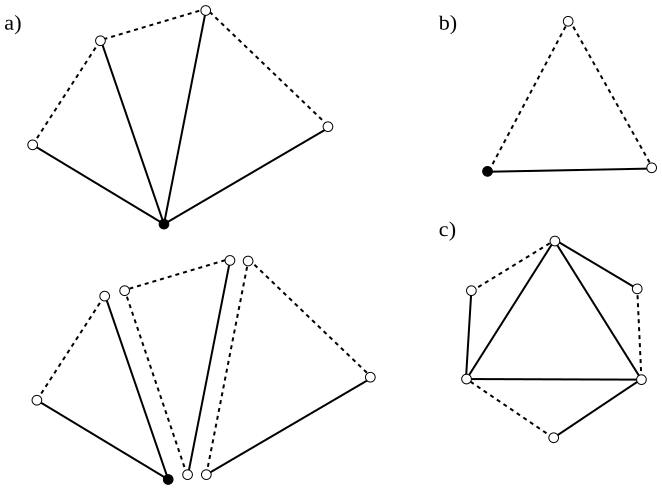
\includegraphics[angle=270,width=4.5in]{partitions}
\caption{a) A partial simplicial complex and a partition of it. Dashed edges are open, solid lines are closed. White vertices are not contained in the complex, but black vertices are. b) A triangle with one closed edge and one vertex is not partitionable. c) A non-partitionable partial simplicial complex. This complex has 0 vertices, 6 edges and 4 triangles. Thus, in a partition, one simplex would need to have at least two closed edges. But then it would also have to contain a vertex, which is impossible.}
\label{fig:partitionability}
\end{figure}

In this section we develop these connections. First, we introduce decision trees as a natural class of scheduling problems that give rise to partitionable allowable configurations. Then, we draw the connection between partitionability and non-negativity of coefficients on the level of polynomials and (nc-)quasisymmetric functions. Finally we discuss important special cases, including generalized permutahedra and $P$-partitions.

Let $\Delta$ be a simplicial complex and assume that $\Delta$ is pure, i.e., that all maximal simplices have the same dimension $k$. A \emph{partition} of $\Delta$ is a map from maximal simplices $\sigma\in\Delta$ to half-open simplices $\hat{\sigma}$ such that $\relint(\sigma)=\relint(\hat{\sigma})$, any two half-open simplicies $\hat{\sigma}_1$, $\hat{\sigma}_2$ are disjoint, and the union of all half-open simplices $\hat{\sigma}$ equals $\Delta$. A partial simplicial complex $\Delta$ is \emph{partitionable} if there exists a partition of $\Delta$. This generalizes the standard notion of partitionability to partial complexes.\footnote{For simplicial complexes, partitionability is often defined in terms of the face poset, which is equivalent to the above definition in terms of half-open simplicies. The face-poset-definition can also be carried over to partial simplicial complexes as follows. Let $\bar{\Delta}$ be the closure of $\Delta$ as defined in Section~\ref{Ehrhart}. Let $\bar{P}$ be the face poset of $\bar{\Delta}$ and let $P$ be the subposet consisting of those faces of $\bar{\Delta}$ whose relative interior is contained in $\Delta$. Then $\Delta$ is partitionable if $P$ can be written as the disjoint union of boolean lattices whose top elements are all at the same height, with respect to $\bar{\Delta}$.} Examples of partitionable and non-partitionable complexes are given in Figure~\ref{fig:partitionability}.

\subsubsection{Decision Trees} Decision trees are a very commonly used form of boolean expression. Intuitively, they are simply nested if-then-else statements. We will work with decision trees where the conditions in the if-clauses are inequalities of the form $x_i \leq x_j$ and the conditions in the leaves of the tree are conjunctions of such inequalities (either strict or weak).

Figure~\ref{fig:tree} shows the example of a decision tree with only one if-then-else statement and the geometric region of points that satisfy the statement.   
\begin{figure}[h]
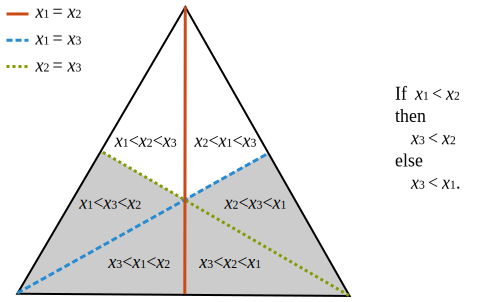
\includegraphics[angle=270,width=3.5in]{simple_decision_tree}
\caption{The allowable configuration associated to the decision tree ``If $x_1<x_2$ then $x_3<x_2$ else $x_3<x_1$,'' shaded in gray, shown as a subconfiguration of the Coxeter complex of type A. Note that the edges of the outer triangle correspond to the inequalities $x_1>0$, $x_2>0$ and $x_3>0$, which are not shown in the boolean formula.}
\label{fig:tree}
\end{figure}
The collection of points $x \in \mathbb{R}^n$ that satisfy the conditions of a tree form a union of faces of the cell decomposition induced by the braid arrangement or equivalently a collection of faces of the Coxeter complex $\cox_A$.  In general, this union of faces can be non-convex (as seen in the Figure) or non star-convex.  Below we show that if a scheduling problem can be expressed as the union of decision trees which satisfy a certain property, then the allowable configuration $\allow(S)$ is partitionable which in turn implies positivity of coefficients for the scheduling functions. 

More formally, decision trees of boolean expressions are defined recursively as follows.

\begin{definition} A \emph{leaf} is a boolean expression $\psi$ that is a conjunction of inequalities of the form $x_i \leq x_j$ or $x_i < x_j$. A \emph{decision tree} is either a leaf, or a boolean expression of the form
\[
  \text{if $\varphi$ then $\psi_t$ else $\psi_f$}
\]
where $\varphi$ is an inequality of the form $x_i \leq x_j$ and $\psi_t,\psi_f$ are decision trees.
\end{definition}

As decision trees are binary trees, it will be convenient to distinguish notationally between a node $v$ of a tree $S$ and the boolean expression $S_v$ at that node.

Every leaf $v$ of a decision tree corresponds to a conjunction of inequalities which we call the \emph{cell} at $v$. The cell at $v$ is the conjunction of $S_v$ (the inequalities given by the leaf $v$ itself) and the constraints given in the if-clauses of ancestors of $v$, negated according to whether $v$ resides in the ``true" or ``false" branch of the corresponding if-then-else clause. Let $v$ denote a leaf of the tree and let $v_0,\ldots,v_k$ denote its ancestors. Then $S_{v_i}$ is a boolean formula of the form ``if $\varphi$ then $\psi_t$ else $\psi_f$'' and we define $\varphi_{v_i}' := \varphi$ if $v$ resides in the branch $\psi_t$ and $\varphi_{v_i}' := \neg\varphi$ if $v$ resides in the branch $\psi_f$. We denote by $C_v$ the conjunction
\[
 C_v := \varphi_{v_0}'\wedge\ldots\wedge\varphi_{v_k}'\wedge S_v\wedge \bigwedge_{i=1}^n (0 < x_i < 1).
\]
By a slight abuse of notation, we will also use $C_v$ to denote the polytope of all $x\in \RR^n$ satisfying $C_v$. In the above formula, the purpose of $\bigwedge (0 < x_i <1)$ is to ensure that all solutions $x$ lie in the open cube $(0,1)^n$, as is usual in the Ehrhart theory setting. When working with quasisymmetric functions, this condition would be replaced, accordingly, with $\bigwedge (0 < x_i)$ so as to ensure that solutions are positive. In this case the solution sets $C_v$ are cones. Note that the set of formulas $\varphi_{v_0}'\wedge\ldots\wedge\varphi_{v_k}'\wedge S_v$ for all leaves $v$ of $S$ correspond exactly to the conjunctions in the disjunctive normal form of $S$.

\begin{figure}[h]
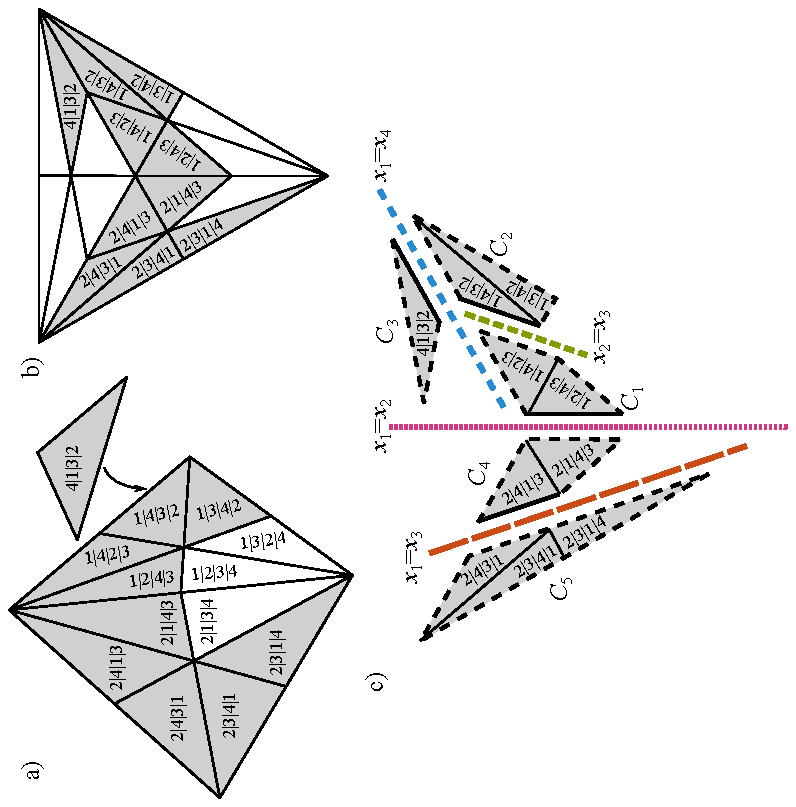
\includegraphics[width=5in,angle=270]{cells.pdf}
\caption{The decision tree described in the text and its cells. a) The front faces of the Coxeter complex, with the faces contained in the allowable configuration of the decision tree shaded in gray. The face $4|1|3|2$ of the allowable configuration lies on the back face of the Coxeter complex. b) A view from above onto the Coxeter complex, showing all faces in the allowable configuration at once. c) The faces of the allowable configuration as partitioned by the decision tree. The cells of the decision tree are the gray components shown in the figure. Dashed lines indicate open faces, while solid lines indicate closed faces. Note that $C_2$ satisfies both $x_1 \leq x_2$ and $x_3 \leq x_2$, however, $x_1 \leq x_2$ is redundant and therefore does not produce a closed facet. }
\label{fig:decision-tree-with-cells}
\end{figure}

To illustrate these definitions, we consider the following example, which is illustrated in Figure~\ref{fig:decision-tree-with-cells}. Let $S$ denote the following decision tree.

\begin{lstlisting}[mathescape,basicstyle=\sffamily\small]
if $x_1\leq x_2$ then
    if $x_1 < x_4$ then
        if $x_2 < x_3$ then $x_4 < x_3$ else ($x_4 < x_2$ and $x_1 < x_3$)
    else
        $x_3 < x_2$ and $x_1 < x_3$
else
    if $x_1 \leq x_3$ then ($x_2 < x_4$ and $x_4 < x_3$) else ($x_1 < x_4$ and $x_2 < x_3$)
\end{lstlisting}

Of course, the same boolean function can be represented by different decision trees. The cells of this decision tree are the following (up to conjuncts of the form $\bigwedge (0 < x_i <1)$ which have been omitted for brevity).
\begin{align*}
C_1 &=& (x_1\leq x_2) \wedge (x_1 < x_4) \wedge (x_2 < x_3) \wedge (x_4 < x_3), \\
C_2 &=& (x_1\leq x_2) \wedge (x_1 < x_4) \wedge (x_3 \leq x_2) \wedge (x_4 < x_2) \wedge (x_1 < x_3), \\
C_3 &=& (x_1\leq x_2) \wedge (x_4 \leq x_1) \wedge (x_3 < x_2) \wedge (x_1 < x_3), \\
C_4 &=& (x_2 < x_1) \wedge (x_1 \leq x_3) \wedge (x_2 < x_4) \wedge (x_4 < x_3), \\
C_5 &=& (x_2 < x_1) \wedge (x_3 < x_1) \wedge (x_1 < x_4) \wedge (x_2 < x_3).
\end{align*}

In the following, we are going to apply some geometric terminology to boolean formulas. A disjunction $\bigvee_i C_i(x)$ is called \emph{disjoint}, if the solution sets are disjoint, i.e., if for every $x$ at most one of the $C_i(x)$ is true. Moreover, the \emph{dimension} of a conjunction $C$ of inequalities is the dimension of the polyhedron of all solutions, i.e, it is the number of variables minus the maximal number of linearly independent equations implied by $C$.

We call a formula $C$ \emph{almost open}, if it is equivalent to a conjunction $\bigwedge_j I_{j}$ of inequalities $I_j$ such that at most one of the $I_j$ is weak and all of the $I_j$ are facet-defining. Note that the $I_j$ are facet-defining if the closure $\bar{C}$ of (the polytope defined by) $C$ has a non-redundant description $\bar{C} = \bigwedge_j \bar{I}_j$, where $\bar{I}_j$ denotes the weak inequality defined by $I_j$. Geometrically, this means that the polytope $C$ is open except for at most one face which may be closed.

In the above example, all cells of the decision tree $S$ are almost open. Note that in $C_2$, the weak inequality $x_1 \leq x_2$ is redundant, whence $C_2$ can equivalently be written as $C_2 = (x_1 < x_4) \wedge (x_3 \leq x_2) \wedge (x_4 < x_2) \wedge (x_1 < x_3)$. Similarly, $C_3$ can be rewritten using only one weak inequality (and two strict inequalities). Note that in Figure~\ref{fig:decision-tree-with-cells} all cells have at most one closed face.

We say a partial polytopal complex is partitionable, if it can be written as the disjoint union of half-open simplicies of full dimension $n$. (In our case, we are of course restricted to use simplicies given by the braid triangulation.)

\begin{theorem}
If a scheduling problem $S$ is equivalent to a formula of the form
\[
  S \equiv \bigvee_i C_i \text{ where } C_i = \bigwedge_j I_{i,j}
\]
where the disjunction is disjoint and the $C_i$ are almost open of dimension $d$, then $\allow(S)$ is partitionable.
\end{theorem}

Because the disjunction is disjoint, this theorem follows immediately, if we can prove it for almost open conjunctions.

\begin{lemma}
\label{lem:almost-open}
An almost open conjunction $C$ of dimension $d$ is partitionable.
\end{lemma}

It is well-known that boundary complexes of simplicial polytopes are partitionable, a fact that can for example be shown using line-shellings \cite{Bruggesser1971}. This method can also be used to construct shellings (and thus partitions) of regular triangulations of polytopes \cite[Corollary~8.14]{Ziegler1995}. These techniques extend naturally to almost open polytopes, as shown in the following proof. For the proof, we assume familiarity with regular triangulations, line-shellings and their connection to partitionability \cite{DeLoera2010,Lee2004,Ziegler1995}.

\begin{proof} 
We first deal with the case where the polytope $C$ has exactly one closed face. Recall that having one closed face means that all but one of the facet-defining inequalities of $C$ are strict.

$C$ is a subconfiguration of the braid triangulation $\TC$ of the open cube, as defined in Section~\ref{sec:allow-forb-configurations}. Therefore, the induced triangulation $T$ of the almost open polytope $C$ is regular. Let $F$ be the facet of $C$ which is closed, and let $z$ denote a new point close to $F$ but outside of $C$. We then create an open polytope $C'$ with $z$ as a new vertex by taking the open convex hull of $C$ and $z$:
\[
  C' = \operatorname{oconv}(C,v) := \mset{\lambda x + (1-\lambda)v}{x\in C, \lambda\in (0,1] }.
\]
Note that $C'$ is open because $(1-\lambda)<1$ and $F$ is the only closed face of $C$. The extended polytope $C'$ then has a triangulation $T'$ which consists of all the simplices in $T$ and the open convex hulls $\operatorname{oconv}(\sigma,z)$ of simplices $\sigma\in T$ such that $\sigma\subset F$ with the new vertex $z$. 

The triangulation $T'$ is regular.\footnote{The new simplices $\sigma\in T'\setminus T$ are separated from $C$ by the hyperplane defining $F$. Moreover $T$ induces a regular triangulation of $F$ and thus the triangulation of $C'\setminus C$ induced by $T'$ is regular as well.} Therefore, there exists a polytope $P$ that has $C'$ as its lower hull. We now construct a line shelling of the lower hull of $P$ which starts with a facet in $T'\setminus T$. The lifted polytope $P$ can be chosen such that that all facets in $T'\setminus T$ are shelled first, again because $T$ is separated from $T'\setminus T$ by a single hyperplane, see also \cite[Lemma~2]{Breuer2011}.

Let $\sigma_1,\ldots,\sigma_N$ be the induced shelling order of the maximal-dimensional simplicies in $C$. Let $\bar{\sigma_i}$ denote the closure of $\sigma_i$. Then, the sequence of half-open simplices
\[
 (\nu_i)_{i=1,\ldots,N}\;  :=\;   \bar{\sigma_1}, \; \bar{\sigma_2}\setminus \bar{\sigma_1}, \; \bar{\sigma_3}\setminus  (\bar{\sigma_2} \cup \bar{\sigma_1}), \; \ldots, \; \bar{\sigma_N} \setminus \bigcup_{i=1}^{N-1} \sigma_i
\]
form a partition of the closed polytope $\bar{C'}$. By reversing which faces of these half-open simplices are open and which are closed, we obtain a partition 
\[
  (\tau_i)_{i=1,\ldots,N}\;  :=\; \bar{\sigma}_N\setminus \partial C' ,\;  \bar{\sigma}_{N-1}\setminus (\partial C' \cup\bar{\sigma}_N),\;  \ldots,\;  \bar{\sigma}_1 \setminus  (\partial C' \cup \bigcup_{i=2}^N \bar{\sigma}_i)
\]
of the open polytope $C'$. Let $\tau_i$ denote the $i$-th element in this sequence, that is, 
\[
  \tau_i = \bar{\sigma}_{N-i+1} \setminus (\partial C' \cup \bigcup_{i=N-i+2}^N \bar{\sigma_i})
\]
for $i=1,\ldots,N$. A face is open if it occurred in a previous simplex of the sequence or the boundary. Because we run through the sequence in reverse order, this flips the state of all faces versus the first partition defined above.

By construction, the simplices in $T'\setminus T$ are the last half-open simplexes in the sequence $(\tau_i)_i$ above, that is, there exists an $l$ such that $\sigma_i\subset C$ for all $i\leq l$ and $\sigma_i\subset C'\setminus C$ for all $i>l$. Then, the sequence $\tau_1,\ldots,\tau_l$ is a partition of $C$, as desired. Note in particular that $\bigcup_{i=1}^l \tau_i$ includes the closed face $F$, precisely because all faces of $C$ come first in the sequence $C$.

This concludes the proof for the case that $C$ has one closed face. The proof for the case that $C$ is an open polytope without closed faces is completely analogous, only simpler as there is no need to add the new vertex $z$.
\end{proof}

\begin{theorem}
\label{thm:decision}
Let $S$ be a decision tree such that all cells of $S$ are almost open of dimension $d$. Then $\allow(S)$ is partitionable. Moreover, disjoint unions of such decision trees are partitionable.
\end{theorem}

\begin{proof} 
A decision tree is the disjoint union of all its cells. By Lemma~\ref{lem:almost-open}, all cells are partitionable because they are almost open. Therefore the decision tree is partitionable.
\end{proof}

Note that a cell can be in the "strict inequality" branch of many of its ancestors and still be almost open. The reason is that, in practice, many of these strict ancestral inequalities will be redundant.

%Note that all theorems stated here hold for $\allowC(S)$ as well as for $\allowP(S)$, with analogous proofs.

\begin{remark}
In general, a partial complex of dimension $k$ is partitionable if it can be written as a disjoint union of half-open simplices of dimension $k$. In the above, we have defined partitionable with respect to the ambient dimension $n$, as this will be convenient when working with the fundamental bases of NCSym and QSym below. However, this restriction is not essential. If $\allow(S)$ can be written as a disjoint union of almost open cells of a fixed dimension $k<d$, then the same proofs show partitionability of $\allow(S)$.
\end{remark}

%% \begin{example}
%% Returning to the chromatic scheduling problem, Theorem~\ref{hilbert}
%% was shown by Steingrimmson in [cite], that $\Sigma(S)$ had a convex
%% ear decomposition by Hersch and Swartz [cite], and L-positivity of the
%% chromatic symmetric function by [cite].  The chromatic scheduling
%% problem can also be seen to satisfy the conditions of
%% Theorem~\ref{posets} and hence Therorem~\ref{unique}.  This was shown
%% in [cite GP] by considering a larger class of scheduling problems
%% defined for generalized permutahedron.  

%% The scheduling problem of [GP] is defined by taking, for each vertex
%% $v$ of a generalized permutahedron $P$, the conjugation of all
%% hyperplanes defining $v$.  Hence the valid $\omega$ schedules
%% correspond to all integer points in the interior of the normal fan or
%% equivalently the forbidden configuration is the entire co-dimension
%% one skeleton $P$.  The normal fans of generalized permutahedron are
%% refined by the braid arrangement and the $C_{i,j}$ of
%% Theorem~\ref{posets} correspond to all interiors of the maximal cones.
%% In cite[GP], the conditions of Theorem~\ref{unique} are established in
%% the Hopf monoid setting of directed faces.  The chromatic scheduling
%% problem is the special instance of the generalized permutahedron
%% scheduling problem for graphical zonotopes.  As another special
%% instance, the quasisymmetric function $QS$ for matroid polytopes is
%% the Biller-Jia-Reiner quasisymmetric function for matroids.
%% \end{example}



\subsubsection{Fundamental Bases for NCQSym and QSym}

%% The scheduling function $\SSS_S$ is a quasisymmetric function in
%% non-commuting variables and $\poly_S(k)$ is a polynomial.  The structure
%% of $\Sigma(S)$ also yields information on the the intermediate
%% quasisymmetric function $QS_S$.

%%   If $\SSS_S$ is given in the monomial
%% bases indexed by ordered set partitions, $QS_S$ is defined as the
%% quasisymmetric function formed by applying the type map to each
%% monomial term.  We will be interested in the expansion of $QS_S$ in
%% bases other than the monomial, in particular the fundamental basis.
%% To this end we review analogous bases in NCQSym which allow us to also
%% specialize via the type map.

Above we established that if a scheduling problem can be written as a
 decision tree such that all cells are almost open then the allowable
configuration is partitionable.  Here we prove that partitionability
of the allowable configuration implies positivity of the scheduling
(nc-)quasisymmetric function in the (nc-)fundamental basis.



 Let $\Phi_\text{c}$ and $\Phi_\text{f}$ (standing for coarse and fine) be two ordered set partitions such that $\Phi_\text{f}$ is a permutation, i.e. an ordered set partition of maximal length into blocks of size one, that refines $\Phi_\text{c}$. Then the poset of all ordered set partitions $\Phi$  between $\Phi_\text{c}$ and $\Phi_\text{f}$ under the refinement relation forms a boolean lattice of dimension $n-\ell(\Phi_\text{c})$ where $\ell$ is the length of $\Phi_\text{c}$. Moreover, the type map gives an isomorphism from this boolean lattice to the boolean lattice of all compositions refining the composition $\operatorname{type}(\Phi_\text{c})$. Thus,
\[
  \ncL_{(\Phi_\text{c};\Phi_\text{f})} := \sum_{\Phi_\text{c}\leq \Phi \leq \Phi_\text{f}} \ncM_\Phi
\]
is an nc-quasisymmetric function $\ncL_{(\Phi_\text{c};\Phi_\text{f})}$ that specializes to $L_{\operatorname{type}(\Phi_\text{c})}$ when the variables are allowed to commute.

As $(\Phi_\text{c};\Phi_\text{f})$ ranges over all such pairs of ordered set partitions, which are comparable under the refinement relation and  where $\Phi_\text{f}$ has length $n$, the functions $\ncL_{(\Phi_\text{c};\Phi_\text{f})}$ form a generating system of the linear space of all nc-quasisymmetric functions. However, they do not form a basis as there are multiple representations of the same function, for example
\[
  \ncL_{(1|2|3;1|2|3)} + \ncL_{(1|23;1|3|2)} =   \ncL_{(1|23;1|2|3)} +  \ncL_{(1|3|2;1|3|2)}
\]
$$ = \ncM_{1|2|3} + \ncM_{1|23} + \ncM_{1|3|2}.$$
We call this the \emph{fundamental generating system} of the nc-quasisymmetric functions. To obtain a basis, we must fix a choice for $\Phi_\text{f}$ given $\Phi_\text{c}$.  In particular, for any ordered set partition $\Phi$, let $\hat{\Phi}$ denote the permutation refining $\Phi$ with the property that the elements of each part of $\Phi$ are listed in order. For example, if $\Phi=35|247|16$ then $\hat{\Phi}=3|5|2|4|7|1|6$. 
Given an ordered set partition, define
 $$\ncL_\Phi:=\ncL_{(\Phi;\hat{\Phi})}.$$ As $\Phi$ ranges over all ordered set partitions, the functions $\ncL_\Phi$ form a basis for the space of nc-quasisymmetric functions, which we call the \emph{nc-fundamental basis}.

Alternatively, this fundamental basis for nc-quasisymmetric functions can be defined in terms of a \emph{directed refinement relation} $\preceq$ on ordered set partitions given by $\Phi \gtrdot (\Phi_i, \ldots,\Phi_{i-1}, \Phi_i \cup \Phi_{i+1}, \Phi_{i+2}, \ldots \Phi_k)$ where every element of the $i$th block is less than every element of the $i+1$th block.  Then, the nc-fundamental basis for NCQSym can be defined by
$$\mathcal{L}_{\Phi} := \sum_{\Psi:\Psi \preceq \Phi} \ncM_{\Phi},$$
where $\Phi$ ranges over all ordered set partitions. 
We note that this order is opposite to the order $\leq_*$ used to define the basis ${\bf Q_{\Phi}}$ in~\cite{Zab}. 
Our choice of ordering is particularly motivated by its connection the the fundamental basis $L$ of QSym; the $\ncL$ basis of NCQSym restricts to the $L$ basis of QSym when the variables are allowed to commute.  

Namely, recall that 
the fundamental quasisymmetric functions of QSym are defined from the monomial quasisymmetric functions as follows.  For any composition $\alpha$, 
$$L_{\alpha} := \sum_{\beta:\beta \textrm{ refines } \alpha} M_{\beta}.$$
The poset of all compositions that refine $\alpha$, ordered by the refinement relation, forms a boolean lattice of dimension $n-\ell(\alpha)$ where $n$ is the total number of elements in the ground set and $\ell$ is the length of $\alpha$. For example, the composition $3+1$ is refined by $1+2+1$, $2+1+1$ and $1+1+1+1$, where $1+2+1$ and $2+1+1$ are incomparable under the refinement relation.



 Applying the type map in the $\ncL$ basis gives the corresponding quasisymmetric function in the $L$ basis in such a way that directed refinement on the level of nc-quasisymmetric functions corresponds to refinement on the level of quasisymmetric functions:

\begin{diagram}[small]
\text{NCQSym } \ncM & \rTo^{\text{ directed refinement }} & \text{NCQSym } \ncL\\
\dTo^{ \type} & & \dTo_{ \type}\\
\text{QSym } M & \rTo^{\text{refinement}} & \text{QSym } L
\end{diagram}

\begin{example}

Consider the nc-quasisymmetric function 
\begin{align*}
 \mathcal{F} & = \ncM_{12|3} + \ncM_{1|23} + \ncM_{1|2|3} + \ncM_{2|1|3} + \ncM_{1|3|2}\\
      & = \ncL_{12|3} + \ncL_{1|23} - \ncL_{1|2|3} + \ncL_{2|1|3} + \ncL_{1|3|2}.
\end{align*}
The corresponding quasisymmetric function; i.e. the quasisymmetric function obtained from $\mathcal{F}$ by allowing the variables to commute is given by
\begin{align*}
 F & = M_{(2,1)} + M_{(1,2)} + 3M_{(1,1,1)}\\
 & = L_{(2,1)} + L_{(1,2)} + L_{(1,1,1)}\\
& = L_{\type(12|3)} + L_{\type(1|23)} - L_{\type(1|2|3)} + L_{\type(2|1|3)} + L_{\type(1|3|2)}.
\end{align*}

\end{example}




%% \subsection{[mostly subsumed, see what needs to be distributed]}


%% For $i=1,\ldots,d+1$, a half-open $d$-dimensional simplex $\Delta$ has precisely $i$ open faces if and only if the minimal dimension of a face of $\Delta$ is $i-1$.\footnote{Here we view $\Delta$ as a partial simplicial complex.} For example, the half-open tetrahedron $\Delta^3_1$ with one open face, can be written as the disjoint union of one open 3-simplex, three relatively open 2-simplices, three relatively open 1-simplices and one (relatively open) vertex. The minimal dimension of a face of $\Delta^3_1$ is therefore $1=3-1-1$. \comment{Todo: Add picture.} Moreover, this minimal face is uniquely determined: it is the unique minimum of the face poset of the partial simplicial complex induced by a half-open simplex. In fact, for $i=0,\ldots,d+1$ the face poset of $\Delta^d_i$ is a boolean lattice of dimension $d+1-i$ with the relatively open $d$-simplex as its maximum and the minimal $(i-1)$-simplex as its minimum. This also works for $i=0$ if we take as the empty face as a minimum, which is of dimension $-1$.

%% In the case of $\TC$, these boolean lattices arise correspond precisely to the boolean lattices we encountered in the definition of $\ncL$ basis for nc-quasisymmetric functions.
Let $\Delta$ be an $n$-dimensional half-open simplex with $i$ open faces, that, as a partial simplicial complex, is a subcomplex of $\TC$. As we have seen above, its faces are in one-to-one correspondence with ordered set partitions. Its minimal $i-1$-dimensional face corresponds to an ordered set partition $\Phi_\text{c}$ of length $i-1$. Its maximal $n$-dimensional face corresponds to an ordered set partition $\Phi_\text{f}$ of length $n$, i.e., a permutation of $n$. The interval of ordered set partitions between $\Phi_\text{f}$ and $\Phi_\text{c}$ corresponds precisely to the face poset of $\Delta$. Therefore, we now immediately have
\[
  \ncL_{(\Phi_\text{c};\Phi_\text{f})}(\mathbf{1}^k) = \ehr_\Delta(k+1) = \binom{k+n-i+1}{n}.
\]

In other words, if $\Phi_{\text{c}}$ is an ordered set partition of length $j=1,\ldots,n$ and $\Phi_{\text{f}}$ is a permutation refining it, then 
\[
  \ncL_{(\Phi_\text{c};\Phi_\text{f})}(\mathbf{1}^k) = \ncL_{\Phi_\text{c}}(\mathbf{1}^k) = \binom{k+n-j}{n}.
\]

This observation extends directly to quasisymmetric functions. Writing $\type(\ncL)$
for the specialization that turns an nc-quasisymmetric function into a quasisymmetric function by allowing variables to commute, we have 
\[
  L_\alpha = \type(\ncL_{\Phi_\alpha}) \;\;\; \text{ and } \;\;\; L_\alpha(\mathbf{1}^k) = \ncL_{\Phi_\alpha}(\mathbf{1}^k) = \binom{k+n-\ell}{n}
\]
for any composition $\alpha$, where $\Phi_\alpha$ denotes any ordered set partition with $\operatorname{type}(\Phi_\alpha) = \alpha$, and $\ell$ is the length of $\alpha$.
We summarize the connections 
 between the fundamental basis of (nc-)quasisymmetric functions and the $h^*$-vector of corresponding polynomials below.

\begin{proposition}
Let $\mathcal{F}$ denote an nc-quasisymmetric function, let $F$ denote a quasisymmetric function and let $p$ denote a polynomial such that
\[
  \type(\mathcal{F}) = F \;\;\; \text{ and } \;\;\; \mathcal{F}(\mathbf{1}^k) = F(\mathbf{1}^k) = p(k).
\]
Namely, $\mathcal{F}$ specializes to $F$ when the variables are allowed to commute and both $\mathcal{F}$ and $F$ specialize to $p$ when the first $k$ variables are set equal to $1$ and the rest to $0$.   Moreover, let $\mu_\Phi$, $\mu_{(\Phi_\text{c};\Phi_\text{f})}$ and $\lambda_\alpha$ denote the coefficient vectors of $\mathcal{F}$ and $F$ in terms of the fundamental bases and let $(0,h^*_1,\ldots,h^*_n)$ denote the $h^*$-vector of $p$,
\begin{eqnarray*}
  \mathcal{F} &=& \sum_\Phi \mu_\Phi \ncL_\Phi = \sum_{(\Phi_\text{c};\Phi_\text{f})} \mu_{(\Phi_\text{c};\Phi_\text{f})} \ncL_{(\Phi_\text{c};\Phi_\text{f})}, \\
  F &=& \sum_{\alpha} \lambda_\alpha L_\alpha,\\
  p(k) &=& \sum_{i=1}^n h^*_i \binom{k+n-i}{n}.
\end{eqnarray*}
Then
\[
  h^*_i 
  = \sum_{\Phi: \ell(\Phi) = i} \mu_\Phi 
  =
   \sum_{\substack{(\Phi_\text{c};\Phi_\text{f}): 
        \\ \Phi_\text{c} \leq \Phi_\text{f}
        \\ \ell(\Phi_\text{c}) = i
        \\ \ell(\Phi_\text{f}) = n
   }} \mu_{(\Phi_\text{c};\Phi_\text{f})}
  = \sum_{\alpha: \ell(\alpha)=i} \lambda_\alpha.
\]
The coefficients $h_i^*$, $\mu_\Phi$, $\mu_{(\Phi_\text{c};\Phi_\text{f})}$ and $\lambda_\alpha$ are integral but may be negative. 

Non-negativity of the $\mu_\Phi$ or the $\mu_{(\Phi_\text{c};\Phi_\text{f})}$ implies non-negativity of the $\lambda_\alpha$, and, in turn, non-negativity of the $\lambda_\alpha$ implies non-negativity of the $h^*_i$.
\end{proposition}


We now return to the geometry of the allowed and forbidden configurations and see that partitionability implies positivity expansions for the fundamental bases and the $h^*$ coefficients. 

%In particular, the theorem holds if $\mathcal{F}=\SSS_S$ is a scheduling nc-quasisymmetric function and $p(k)=\poly_S(k)$ is the corresponding scheduling polynomial.

%% \begin{proof}
%% We have $\mathcal{F}(\mathbf{1}^k)=F(\mathbf{1}^k)=p(k)$. Moreover, we have seen that 
%% \[
%%   \ncL_{(\Phi_\text{c};\Phi_\text{f})}(\mathbf{1}^k) = L_\alpha(\mathbf{1}^k)=\binom{k+n-i}{n}
%% \]
%% where $i$ denotes the length of $\Phi_\text{c}$ and $\alpha$, respectively. The length of an ordered set partition of $[n]$ or, respectively, an ordered partition of $n$ can range from $1$ to $n$. By collecting terms in each case, we obtain the theorem. Note that the coefficients in the fundamental basis are integral because the coefficients in the monomial basis are integral for any scheduling problem.
%% \end{proof}

%%  \comment{Todo: Add examples/citations.} One class of theorems of this type are phrased in terms of partitionability, which we can generalize for our purposes.

%% A pure partial simplicial complex $K$ is \emph{partitionable} if $K$ can be written as a disjoint union of half-open full-dimensional simplicies. This corresponds to decomposing the face poset of $K$ into boolean lattices whose minimal and maximal elements correspond to the pairs $(\Phi_{\text{c}};\Phi_{\text{f}})$ we discussed above.

\begin{theorem}
\label{thm:part-pos}
Let $S$ be a scheduling problem such that $\allow(S)$ is partitionable. Then there exists a representation
\[
  \SSS_S = \sum_{(\Phi_\text{c};\Phi_\text{f})} \mu_{(\Phi_\text{c};\Phi_\text{f})} \ncL_{(\Phi_\text{c};\Phi_\text{f})}
\]
with non-negative coefficients $\mu_{(\Phi_\text{c};\Phi_\text{f})}\in \{0,1\}$. In particular, 
the scheduling quasisymmetric function is $L$-positive and the scheduling polynomial is $h^*$-positive.
\end{theorem}
\begin{proof}
As $\allowC(S)$ is partitionable, there exists a collection $C$ of half-open $n$-dimensional simplices $\sigma\in\TC$ such that $\allowC(S)=\bigcup_{\sigma\in C}\sigma$ and this union is disjoint. Each element $\sigma\in C$ corresponds to a distinct pair $(\Phi_\text{c};\Phi_\text{f})$ of ordered set partitions, where $\Phi_\text{f}$ refines $\Phi_\text{c}$ and $\Phi_\text{f}$ has length $n$. Let $P$ denote the collection of all pairs corresponding to half-open simplices in $C$. Then
\[
  \SSS_S = \sum_{(\Phi_c;\Phi_f)\in P} \ncL_{(\Phi_c;\Phi_f)}
\]
as desired. The non-negativity of the coefficients of the scheduling quasisymmetric function in the fundamental basis and the $h^*$-vector of $\poly_S$ is implied by the existence of a non-negative representation of $\SSS_S$ in the fundamental generating system.
\end{proof}

\begin{corollary}
Let $S$ be a scheduling problem expressable as a union of decision trees with all cells almost open, then the scheduling quasisymmetric function is $L$-positive and the scheduling polynomial is $h^*$ positive. 
\end{corollary}
\begin{proof}
This is an immediate consequence of Theorems~\ref{thm:part-pos} and~\ref{thm:tree-part}.
\end{proof}
Note that, conversely, the existence of a representation of $\SSS_S$ with 0-1 coefficients in terms of the fundamental generating system implies that $\allow(S)$ is partitionable. However, the same is not true of the coefficients of the scheduling polynomial or quasisymmetric function.  There are scheduling problems where $h^*(\poly_S)$ is non-negative but $\allow(S)$ is not partitionable. 

The next theorem guarentees positivity of the nc-quasisymmetric scheduling function $\SSS$ in terms of the directed refinement relation.


\begin{theorem}
\label{unique}
Let $S$ be a scheduling problem such that $\allow(S)$ is closed under the directed refinement relation. If for every $\Phi \in \allow(S)$ there exists a \emph{unique} coarsest allowed ordered set partition $\Phi_c \preceq \Phi$ such that $\Phi$ is a directed refinement of $\Phi_c$, then the coefficients of $\SSS_S$ in terms of the fundamental basis as well as the $h^*$-vector of $\poly_S$ are non-negative.
\end{theorem}

\begin{proof}
For any  ordered set partition $\Phi_f \in \allow(S)$ of length $n$, there exists by assumption a unique coarsest allowed ordered set partition $\Phi_c$ with $\Phi_c\preceq\Phi_f$. Let $P$ be the collection of all such pairs.  Since $\allow(S)$ is closed under the directed refinement relation, the intervals  $[\Phi_c, \Phi_f]$ are boolean lattices.
% Thus, the interval between $\Phi_c$ and $\Phi_f$ under the directed refinement relation coincides with the interval between $\Phi_c$ and $\Phi_f$ under the ordinary refinement relation. Because of
% The uniqueness assumption guarentees these intervals are disjoint. Finally, again because of the assumption that the allowed poset is closed under directed refinement and has unique coarsest elements, we have that 
Furthermore,  for any  $\Phi \in \allow(S)$ there exists a $\Phi_f$ of length $n$ that is a directed refinement of $\Phi$, hence $\Phi$ is contained in the interval with $\Phi_f$ as its maximal element. Therefore, $P$ forms a partition of $\allow(S)$  which completes the proof of the theorem.
\end{proof}


Note that the condition that $\allow(S)$ is closed under the directed
refiement relation is equivalent to the requirement that the forbidden
configuration $\forb(S)$ be a valid subcomplex of the Coxeter complex; i.e. a
collection of faces closed under taking subsets.


\subsubsection{Disjunction of Conjunctions}
An important class of scheduling problems that satisfy the conditions of Theorem~\ref{unique} are those scheduling problems that can be expressed as a disjunction of conjunctions of strict inequalities, i.e.,
\[
  S = \bigvee_i C_i \text{ where } C_i = \bigwedge_j I_{i,j}
\] \label{posets}
such that the $I_{i,j}$ are strict inequalities of the form $x_a <
x_b$ for some $a$ and $b$, and the conjunctions $C_i$ are satisfiable
for all $i$.  Equivalently, the regions of $[0,1]^n \, \backslash \,
\forb(S)$ are interiors of convex polytopes of dimension $n$.  Such
scheduling problems are a special case of
decision trees with all cells fully open.  Therefore, Theorem~\ref{thm:part-pos} already
provides $\ncL$-positivity, but the conditions of
Theorem~\ref{unique} are easier to interpret in this case.  The
$C_i$ are conjunctions of strict inequalities. Geometrically, the
allowable schedules given by a $C_i$ form a cone; the intersection of
halfspaces defined by the inequalities $x_a < x_b$.  On the Coxeter
complex, such regions are known as posets of the complex.  In particular, let $C_i =
\bigwedge_j I_{i,j}$, the inequalities $I_{i,j}$ naturally induce a
partial order on $[n]$.  The collection of facets of the Coxeter
complex contained in the cone corresponding to $C_i$, thought of as
permutations, consist of all possible linear extensions of the partial
order.  The partial orders corresponding to the $C_{i,j}$ yield the unique coarsest allowable ordered set partitions.


\begin{example}
Suppose $C = (x_1 < x_2) \wedge (x_1 < x_3) \wedge (x_3 < x_4)$.  The corresponding poset $P$ is given in Figure~\ref{fig:poset}(a).  The linear extensions of $P$ are $\{1234, 1324, 1342\}$ and the corresponding cells of $\cox_A$ are shaded in Figure~\ref{fig:poset}(b).
\end{example}

\begin{figure}[h]
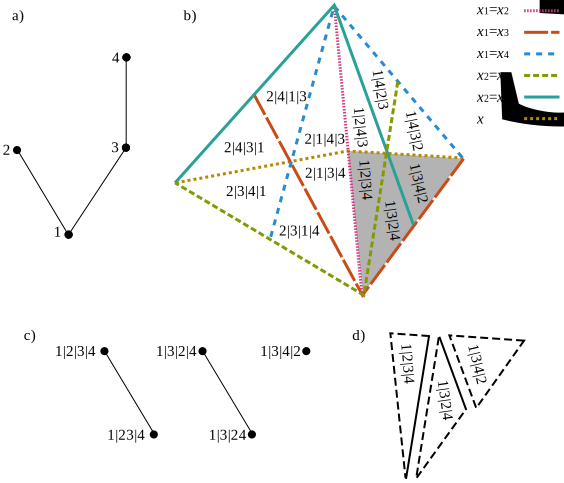
\includegraphics[angle=270,width=5in]{coxeter_complex_poset}
\caption{A poset corresponds to a convex region in the Coxeter complex $\cox_A$, given by a conjunction of inequalities.}
\label{fig:poset}
\end{figure}

The case of a disjunction of conjunctions includes the coloring complex regarded as the forbidden
subcomplex of the graph coloring problem.  Again recall that the
coloring complex can be interpreted as all those ordered set
partitions of the vertices such that at least one block contains at
least one edge.  Let $G=(V,E)$ be a graph on $n$ vertices.  The
graphical arrangement $\mathcal{A}_G$ associated to $G$ is the
subarrangement of the braid arrangement consisting of the hyperplanes
$\{x_i = x_j | \, i,j \in E\}$. The graphical zonotope ${P}_G$ is the
zonotope dual to this arrangement formed by the sum of all normals to
all planes in the arrangement.  Geometrically, this leads to a
perspective first noted explicitly by Hersh and Swartz: the coloring
complex of $G$ is the codimension one skeleton of the normal fan of ${P}_G$
as subdivided by the Coxeter complex~\cite{HS}.  Equivalently, as a scheduling problem,  the
allowable configuration consists of all integer points in the
interiors of maximal cones of the normal fan.  These interiors are
conjunctions of strict inequalities, one for each facet defining
hyperplane of the cone.  In this case, the disjunction is then over
all cones in the fan.

\begin{example}
Consider the complete graph on $3$ vertices, $K_3$.  Any coloring of
$K_3$ must give distinct colors to each vertex.  Figure~\ref{fig:normalfan} shows
the graphical zonotope associated to $K_3$ and it's normal fan.  The
$6$ maximal cones of the fan correspond to the $6$ ordered set
partitions which place the vertices in distinct blocks.

$$\textrm{Chromatic NCQSym}(K_3) = \ncM_{1|2|3} +\ncM_{2|1|3} +\ncM_{2|3|1} +\ncM_{1|3|2} +\ncM_{3|1|2} +\ncM_{3|2|1},$$ 
$$\textrm{Chromatic QSym}(K_3) = 6M_{(1,1,1)},$$
$$\chi(K_3) = k(k-1)(k-2).$$

\end{example}



\begin{figure}[h]
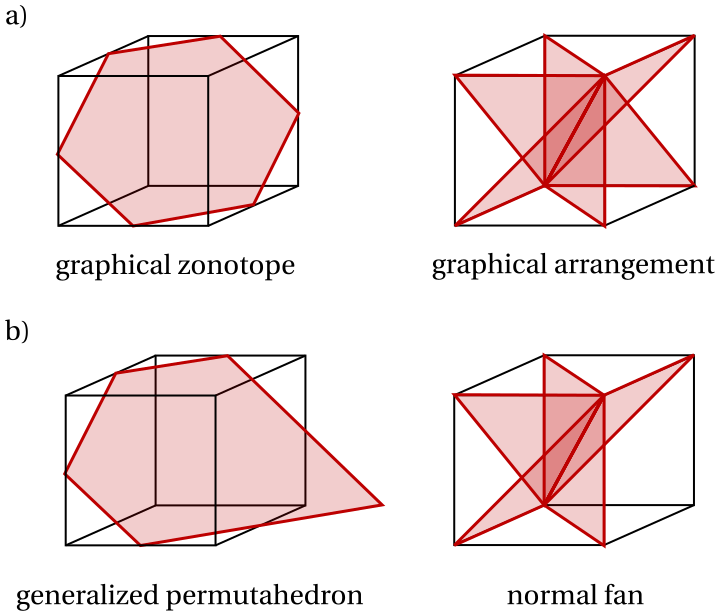
\includegraphics[angle=270,width=4in]{zonotope_and_generalized_permutahedron}
\caption{a) The graphical zonotope of the complete graph $K_3$ and the corresponding graphical arrangement. b) A generalized permutahedron and its normal fan.}
\label{fig:normalfan}
\end{figure}


In~\cite{ABK}, this construction was extended from graphical zonotopes to all generalized
permutahedron.   Generalized permutahedron are typically
defined as the class of polytopes in $\mathbb{R}^n$ such that every
edge is parallel to $e_i - e_j$ for some $i,j \in [n]$.  An equivalent
characterization of generalized permutahedron is the following.
\begin{proposition}\cite{PRW,MPSSW}
 A
polytope is a generalized permutahedron if and only if its normal fan
is refined by the braid arrangement.
\end{proposition}
  Hence the
graphical zonotope, dual to a subarrangement of the braid arrangement,
is a generalized permutahedron.  Other examples include matroid
polytopes, associahedra, and graph associahedra.  A scheduling problem
$S$ can be associated to any generalized permutahedron $GP$ by
defining the forbidden configuration $\forb(S)$ to be the codimension
one skeleton of the normal fan of $GP$ as subdivided by the Coxeter
complex.  Such a scheduling problem is then given as a disjunction of
conjunctions.  Namely, the scheduling problem of a generalized
permutahedron is defined by taking, for each vertex $v$ of a
generalized permutahedron $GP$, the conjunction of all hyperplanes
defining $v$.  Hence the valid  schedules correspond to all
integer points in the interior of the normal fan.  In~\cite{ABK}, this allowable configuration and nc-quasisymmetric funciton were studied not as a schedulign problem but in connection to the Hopf monoid of generalized permutahedron.  There it
was shown that the  generalized permutahedron nc-quasisymmetric function is $\ncL$
positive and $\forb(S)$ is $h$-positive.




Returning to the graphical case, again in~\cite{HS}, this perspective of the normal fan is used to prove that the coloring
complex has a convex ear decomposition which implies strong relations on
the chromatic polynomial. The authors consider the generalization of their result from chromatic polynomials of graphs to characteristic polynomials of matroids.
 They note empirically
however that their results do not seem to generalize.  The perspective
here suggests that the generalization should not be from chromatic
polynomials to characteristic polynomials, but from the scheduling
polynomials of graphic zonotopes to the scheduling polynomials of
matroid polytopes.  Namely, to scheduling problems whose forbidden
configuration is the codimension one skeleton of the normal fan of a
matroid polytope  (and more generally to any generalized permutahedron).  The corresponding scheduling polynomial for matroid polytopes is the
polynomial restriction of the Billera-Jia-Reiner quasisymmetric
function for matroids~\cite{BJR}.

%Talk about previous results on quasisymmetric function positivity.

%% \begin{theorem} \label{unique} Let $S$ be a scheduling problem on $d$ items.  If the forbidden configuration $\Sigma(S)$ is a subcomplex of the Coxeter complex and if for each total ordering of $[d]$ there is a unique coarsest schedule satisfying $S$, then $\SSS_S$ is $\ncL$-positive and therefore $QS$ is $L$-positive. 
%% \end{theorem}

%% Let $S$ be a scheduling problem such that the regions of $[0,1]^n\setminus\Sigma(S)$ are the interiors of convex polytopes of dimension $n$. Equivalently, we assume $S$ can be written as a disjunction of conjunctions of strict inequalities, i.e.,
%% \[
%%   S = \bigvee_i C_i \text{ where } C_i = \bigwedge_j I_{i,j}
%% \] \label{posets}
%% such that the $I_{i,j}$ are strict inequalities of the form $x_a < x_b$ for some $a$ and $b$, and the conjunctions $C_i$ are satisfiable for all $i$.
%% \begin{example}
%% Returning to the chromatic scheduling problem, Theorem~\ref{hilbert}
%% was shown by Steingrimmson in [cite], that $\Sigma(S)$ had a convex
%% ear decomposition by Hersch and Swartz [cite], and L-positivity of the
%% chromatic symmetric function by [cite].  The chromatic scheduling
%% problem can also be seen to satisfy the conditions of
%% Theorem~\ref{posets} and hence Therorem~\ref{unique}.  This was shown
%% in [cite GP] by considering a larger class of scheduling problems
%% defined for generalized permutahedron.  

%% The scheduling problem of [GP] is defined by taking, for each vertex
%% $v$ of a generalized permutahedron $P$, the conjugation of all
%% hyperplanes defining $v$.  Hence the valid $\omega$ schedules
%% correspond to all integer points in the interior of the normal fan or
%% equivalently the forbidden configuration is the entire co-dimension
%% one skeleton $P$.  The normal fans of generalized permutahedron are
%% refined by the braid arrangement and the $C_{i,j}$ of
%% Theorem~\ref{posets} correspond to all interiors of the maximal cones.
%% In cite[GP], the conditions of Theorem~\ref{unique} are established in
%% the Hopf monoid setting of directed faces.  The chromatic scheduling
%% problem is the special instance of the generalized permutahedron
%% scheduling problem for graphical zonotopes.  As another special
%% instance, the quasisymmetric function $QS$ for matroid polytopes is
%% the Biller-Jia-Reiner quasisymmetric function for matroids.
%% \end{example}


\subsubsection{P-partitions} Scheduling problems that can be written as a disjunction of conjunctions  can be
described in terms of $P$-partitions for posets $P$ with all strict
edges.  Again, each $C_{i,j}$ is a collection of strict edges of the
form $x_a < x_b$ which defines a poset.  The scheduling quasisymmetric function
 restricted to a single $C_{i,j}$ is the generating function
$K_{(P,\omega)}$ where $\omega$ is a ``fully un-natural'' labelling of
$P$.  For schedules with a single $C_{i,j}$, Theorem~\ref{unique}
gives a special case of Stanley and Gessels~\cite{Gessel,StanP} 
%the Fundamental theorem of quasisymmetric functions, i.e. the
expansion of $K_{(P,\omega)}$ in the fundamental basis by descent
sets.  In this case, with all strict labels, the unique coarsest
elements for each ordering can also be defined by the descent sets.


Theorem~\ref{unique} is neither  stronger nor weaker than the
$K_{(P,\omega)}$ expansion.  Posets with non-strict edges may easily
be non-positive in the $\ncL$ basis and many scheduling problems
satisfy the conditions of Theorem~\ref{unique} but do not arise from
any poset or P-partition structure as seen in the example below.

\begin{example} 
Consider the scheduling nc-quasisymmetric function,

\begin{align*}
\SSS_S & = \ncL_{24|13} + \ncL_{4|2|13} + \ncL_{24|3|1} + \ncL_{2|14|3} + \ncL_{2|1|34} + \ncL_{4|2|3|1}\\
& = \ncM_{24|13} + \ncM_{2|4|13} + \ncM_{24|1|3} + \ncM_{2|4|1|3} + \ncM_{4|2|13} + \ncM_{4|2|1|3} + \ncM_{24|3|1}\\
& + \ncM_{2|4|3|1} + \ncM_{2|14|3} + \ncM_{2|1|4|3} + \ncM_{2|1|34} + \ncM_{2|1|3|4} + \ncM_{4|2|3|1}.
\end{align*}

The corresponding scheduling problem $S$ does satisfy the conditions of Theorem~\ref{unique}, i.e for every allowable ordered set partition $\Phi$ there is a unique coarsest ordered set partition $\Phi_c$ below $\Phi$ in the directed refinement ordering.  On the other hand, $S$ can not be written as the conjunction of disjunctions.


\end{example}




%% \subsubsection{Convex ear decompositions and strong bounds on the coefficients}

%% \comment{Perhaps this subsection will not explicitly define all the neccesary material but will be written in the form of ``for the knowledgable'' reader, the following ideas work....}

%% \comment{Under construction}

%% \begin{proposition}
%% Let $S$ be a scheduling problem such that $\Sigma(S)$ is of codimension 1 and has a convex ear decomposition. Then 
%% \[
%%   \sum_{n \geq 0} ((n+1)^d - \poly_S(n+1)) t^n = \frac{h_{\Sigma(S)}(t)}{(1-t)^d},
%% \]
%% as above, and moreover the coefficients $h_i$ satisfy
%% \begin{enumerate}
%% \item $h_0 \leq h_1 \leq \ldots \leq h_{\floor{d/2}}$,
%% \item $h_i\leq h_{d-i}$ for $i\leq d/2$,
%% \item $(h_0,h_1-h_0,h_2-h_1,\ldots,h_{\ceil{d/2}}-h_{\ceil{d/2}-1})$ is an $M$-vector.
%% \end{enumerate}
%% \end{proposition}


\subsection{Subcomplexes and the Co-fundamental basis}
\label{sec:cofundamental}


We have seen how particular niceness conditions on the allowable
configuration $\allow(S)$ and the forbidden configuration $\forb(S)$
translate into strong properties of the expansions of scheduling nc-quasisymmetric and quasisymmetric functions  in the fundamental bases and the relationship between the
$h$-vectors of these complexes and the polynomial restriction
$\poly(S)$. 
 In particular, many special cases above resulted in
$\forb(S)$ being a valid subcomplex of the Coxeter complex (as
opposed to simply a collection of faces). This was the case for example for the chromatic scheduling problem and more generally the generalized permutahedron scheduling problem. 
 Here we consider scheduling problems such that $\allow(S)$ is a valid
 subcomplex of $\cox_A$, i.e. the ordered set partitions satisfying
 $S$ are closed under coarsening.  In this case, expansion in the
 fundamental basis is not a natural choice.  Expansion in the
 co-fundamental basis, however, is natural and does yield good
 behavior. 

 The co-fundamental basis for quasisymmetric functions is
 defined analogously to the fundamental basis with refinement replaced by coarsening.  Namely, for a fixed composition $\alpha$, define $N_{\alpha}$ as the sum over all monomials indexed by compositions that coarsen $\alpha$,
$$N_{\alpha} := \sum_{\beta : \beta \, \textrm{coarsens} \, \alpha} M_{\beta}.$$
The co-fundamental basis given by the $N_{\alpha}$ also results from allowing the variables to commute in the NCQSym basis ${\bf {Q}_{\Phi}}$ defined in~\cite{Zab}.



 %%   We will use the notation $\ncN_{\Phi}$ for the basis which sums
 %%   over all ordered set partitions that \emph{coarsen} a fixed
 %%   partition with respect to a fixed direction and refer to it as the
 %%   co-nc-fundamental basis.  This basis was introduced in~\cite{Zab} and denoted *.  It is precisely opposite the directed refinement relation defined for the findamental basis.   Namely,
 %% $$\ncN_{\Phi} := \sum_{\Psi:\Phi \preceq \Psi} \ncM_{\Phi}.$$
 %% Again, after applying the type map to the indexing ordered set partitions, we arrive at a quasisymmetric expansion in terms of all compositions that coarsen a fixed composition. 


  Recall that for an integer point $a\ \in \mathbb{N}^n$,
  $\Delta(a)$ is the ordered set partition recording the relative
  ordering of components of a; i.e. $a$ is constant on each $\Delta_i$
  and satisfies $a|_{\Delta_i} < a|_{\Delta_{i+1}}$ for all $i$.
Given an integer point $a$ or an ordered set partition $\Delta(a)$ we now associate a flag:
$$\mathscr{F}_{a} = \mathscr{F}_{\Delta(a)} := F_0 \subset F_1 \subset \ldots \subset F_k := [n]$$
such that $a$ is constant on each set $F_i - F_{i-1}$ and  $a|_{F_i -
  F_{i-1}} < a|_{F_{i+1} - F_{i}} $. 

\begin{example}
Suppose $a$ is an integer point satisying $a_2 < a_1 = a_3 = a_4$ then $\Delta(a) = (2|134)$ and $\mathscr{F}_{\Delta(a)} = {\emptyset \subset \{2\} \subset \{1,2,3,4\}}$.
\end{example}



Given a scheduling problem, if the allowable configuration corresponds
to the collection of all flags of a graded poset, then clearly $\allow(S)$ is closed under coarsening.  In this case, the scheduling 
quasisymmetric function has a particularly nice expansion.

\begin{proposition}
\label{prop:flags}
Let $S$ be a scheduling problem such that the collection of flags corresponding to the elements of $\allow(S)$,
$$\{ \mathscr{F}_{\Delta(a)} \, | \, \Delta(a) \in \allow(S) \},$$
forms the collection of all flags of a graded poset.  Then the coefficient of $N_{\alpha}$ in the expansion of scheduling quasisymmetric function in the co-fundamental basis is given by:
$$[N_{\alpha}] = (-1)^{|\alpha|} \sum_{\alpha \, \textrm{flags}} \prod_i \mu(f_i,f_{i+1})$$
where an $\alpha$-flag is a flag such that $|f_{i+1}| - |f_i| = \alpha_i$ and $\mu$ is the M\"{o}bius function of the poset.
\end{proposition}



Proposition~\ref{prop:flags} associates a quasisymmetric function to a
graded poset.  The allowable flags are all chains in the poset.  Thus,
in the monomial basis, the scheduling quasisymmetric function is indexed
by compositions recording the \emph{size} of each step in the flag.  This
quasisymmetric function is very similar to but not the same as
Ehrenborg's quasisymmetric function associated to graded
posets~\cite{Ehrenborg}.  For any graded poset $P$, Ehrenborg defines
a quasisymmetric function $F(P)$ by summing over all chains of the
poset and recording the \emph{rank jump} of the flag at each step.  Although
the quasisymmetric functions record different data from the poset, our
Proposition~\ref{prop:flags} is equivalent to
~\cite[Proposition~5.1]{Ehrenborg}, where our expansion in the
co-fundamental basis is equivalent to his expansion of the image of
the Malvenuto and Reutenauer involution of quasisymmetric functions.
The equivalence is seen by noting that the coefficients are given by a
manipulation of the M\"obius function, and the compositions indexing the
monomials could be any collection of compositions associated to a
chain that is closed under coarsening.




\subsubsection{The Bergman scheduling problem} As an explicit example of Proposition~\ref{prop:flags} we consider the Bergman
scheduling problem, so named because the lattice points of the
allowable configuration are precisely those contained in the Bergman
fan of a matroid. In this case, the scheduling polynomial is the
Zeta-polynomial of the matroid.

Let $M$ be a matroid on ground set $E$ and let $\omega \in
\mathbb{N}^{|E|}$.  Consider $\omega$ as a weight function on the ground
set of $M$ and define the weight of a basis $B$ to be: $\omega(B) =
\sum_{e\in B} \omega(e)$.  The Bergman fan is defined to be  all
$\omega$ such that every element of $M$ is in some basis of minimal $\omega$-weight.  Note that if $\omega$ is in the Bergman fan, then so are all
weight functions with the same relative ordering.  Hence, we can
define the Bergman scheduling problem to be the scheduling problem
whose allowable configuration is given by the integer points of the
Bergman fan.
%%  Furthermore define $M_{\omega}$ to be the induced matroid of all
%% $\omega$-minimal bases. 
%% % Three different perspectives on this induced
%% %matroid and that fact that it is indeed a matroid are discussed in~\cite{AK, Section 2}.
%% The function $\omega$ is called $M$-loopless if the matroid
%%   $M_{\omega}$ has no loops, i.e.  every element of the ground set is
%%   contained in some minimal weight basis.  In~\cite{AK}, such $\omega$ are
%%   called valid and precisely constitute the integral points of the
%%   Bergman fan of $M$.
  Considering $\omega$ simply as an integer
  point, we associate a flag $\mathscr{F}_{\omega}$ as above.
In ~\cite{AK} it is shown that a weight function $\omega$ is  in the Bergman fan
if and only if $\mathscr{F}(\om)$ is a flag of flats of $M$.
%% $M_{\omega}$ is completely determined by the relative ordering of the
%%   componants of $\omega$ and not their exact value, hence we make the
%%   following definitions.
Therefore, the Bergman scheduling problem is the scheduling problem with allowable configuration $\allow(S)$ equal to all $\Delta(\om)$ such that $\mathcal{F}_{\omega}$ is a flag of flats of $M$. 

%% $\om$ is $M$-loopless.  The Bergman nc-quasisymmetric function is the generating function,
%% $$NCQB(M,{\bf x}) := \sum_{M\textrm{-loopless} \, \omega} {\bf x}_{\omega},$$
%% where ${\bf x}_{\omega} = \prod_{e \in E} x_{\omega(e)}$.

\begin{example}

Let $U_{2,4}$ be the uniform matroid of rank $2$ on a ground set of
size $4$.  
$$\textrm{Bergman QSym}(U_{2,4})  = {\ncM}_{1234} + {\ncM}_{1|234} + {\ncM}_{2|134} + {\ncM}_{3|124} + {\ncM}_{4|123}. $$

The presence of the term ${\ncM}_{1|234}$, for example, reflects that any $\omega$ such that $\omega_{i_1} < \omega_{i_2} =
\omega_{i_3} = \omega_{i_4}$ yields the minimum weight bases:
$\{12,13,14\}$.  Alternatively, $\{ 1 \subset 1234\}$ is a flag of
flats.  The contribution to Bergman QSym$(U_{2,4})$ will be $M_{(1,3)}$ since $(1,3)$
is the image of the ordered set partition under the type map.
Ehrenborg's quasisymmetric function would instead record the rank jumps of this flag giving a contribution of $M_{(1,2)}$.


\end{example}

%% \begin{theorem}\label{thm:Bergman}[Theorem 1 ref]
%% A weight function $\omega$ is $M$-loopless if and only if $\mathcal{F}(\om)$ is a flag of flats of $M$.
%% \end{theorem}


%% Applying the type map to NCQBergman gives the quasisymmetric
%% function QBergman, 
%% $$QB(U_{2,4}) = M_4 + 4M_{1,3}.$$


The collection of ordered set partitions which index the Bergman
nc-quasisymmetric function are closed under {\em coarsening} and moreover form the collection of flags of the lattice of flats of the matroid. Therefore Proposition~\ref{prop:flags} implies that the coefficients of the Bergman quasisymmetric function in the co-fundamental basis are given by
%% \begin{proposition} For the Bergman scheduling problem $S$, the coefficients of the quasisymmetric function QSym(S) in the cofundamental basis satisfy:
%% \begin{enumerate}
%% \item
$$[N_{\alpha}] = (-1)^{|\alpha|} \sum_{\alpha \, \textrm{flags}} \prod_i \mu(f_i,f_{i+1}),$$
where an $\alpha$-flag is a flag of flats such that $|f_{i+1}| - |f_i| = \alpha_i$ and $\mu$ is the M\"{o}bius function of the lattice of flats of $M$.  The lattice of flats of a matroid is a well studied object and allows us to further understand these coefficents.  For example, the sign of $[N_{\alpha}]$ alternates with the length of $\alpha$,  $\sum_{\alpha} [N_{\alpha}] = 1$, and up to sign, $ [N_{|E|}]$ is equal to the Mobius function of the lattice
of flats $\mu(0,1)$ or equivalently the reduced Euler characteristic of the order complex of the
proper part of the lattice of flats.


%% \begin{proof}
%% \begin{enumerate}
%% \item This is an immediate corollary of Proposition~\ref{prop:flags}.
%% \item  In any composition of $n$, the parity of the number of odd parts is the same.
%% \item  Alternating sum over subsets
%% \item (It is the alternating sum of the f-vector just broken up by the refinement).
%% \end{enumerate}
%% \end{proof}

\begin{example}


%% The Bergman quasisymmetric functions of the uniform matroids of rank $2$ and $3$ on a ground set of size $3$ and $4$:

%% \begin{align*}
%% QB(U_{2,4}) & = M_4 + 4M_{1,3}\\
%% & = 4N_{1,3} - 3N_4
%% \end{align*}

%% \begin{align*}
%% QB(U_{3,4}) & =  M_4 + 6M_{2,2} + 4M_{1,3} + 12M_{1,1,2}\\
%%             & =  12 N_{1,1,2} - 8 N_{1,3} - 6N_{2,2} + 3N_4
%% \end{align*}
The Schubert matroid $M_{(135)}$ is the matroid consisting of 
all bases componentwise less than or equal to $(1,3,5)$.  The Bergman quasisymmetric function is given by $ \textrm{Bergman QSym}(M_{(135)})$ 
\begin{align*}
&  =  M_5 + 3M_{2,3} + M_{3,2} + M_{4,1} + 3M_{1,4}  + 4M_{1,1,3} + M_{1,2,2} + M_{2,1,2} + M_{2,2,1} + 2M_{1,3,1}\\
&  =  2N_{1,3,1} + N_{2,2,1} + N_{2,1,2} + N_{1,2,2} + 4N_{1,1,3}  - 4 N_{1,4} - 2N_{4,1} - N_{3,2} - 3N_{2,3} + 2N_5.
\end{align*}

\end{example}


%%  If we were working over rank instead of size, we would have the
%%  Ehrenborg quasi-symmetric function which runs over flags of flats
%%  indexed by rank (as in the lattice).

%%  The $\eta$s are a colored refinement of a ``co-h'' vector of the
%% order complex.  The ``co-h'' is computed via Stanley's trick with the
%% $f$-vector written backwards from the top down the right hand side and
%% $f_n$ down the left hand side.

%% The coefficients $(f_{\beta_1}f_{\beta_2} \dots f_{\beta_n})$ are
%% a colored refinement of the $f$-vector of the order complex of the
%% lattice of flats. Flats of the same size (NOT RANK) are given the same
%% color.


%\comment{See Richard's result on chromatic in the power sum basis, alternates in sign by length of partition.}

%It might be hard to recognize, but see proposition 5.1 which is really the same as the proposition above interpreted via the antipode formula for a Hopf algebra. 



The Bergman polynomial obtained
by evaluating at ${\bf 1}^k$ counts the number of
$k$-schedules satisfying the boolean formula prescribed by the closure
operator. 

\begin{proposition}
The Bergman polynomial of a matroid is equal to the zeta polynomial of the lattice of flats of the matroid, which counts multichains of length $k$ in the lattice,
$$\textrm{Bergman QSym}(M;{\bf 1}^k) = Z(L(M),k) = |\{ \hat{0} = y_0 \leq y_1 \leq \cdots \leq y_k = \hat{1} | y_i \in L(M) \}|.$$

\end{proposition}

 One could interpret the rank as a kind of cost function -
once certain jobs are started, others of the same rank can be added
without additional cost.  To minimize cost, we require that in any
scheduling of jobs, at each time step we have a closed subset of jobs.

\begin{example}
Returning to the example of $U_{2,4}$, the Bergman polynomial is
$$\textrm{Bergman QSym}(U_{2,4};{\bf 1}^k) = 2k^2 - k.$$

The flats of this matroid are all singletons and the entire set [4].  In terms of scheduling, any job may be started first and then all others must be started simultaneously.  Alternatively, all jobs may be started at the same time, but we do not allow for only two jobs to start at the same time. 
\end{example}






%% \subsection{Reciprocity theorems}

%% \begin{theorem}\label{posets}
%% Let $S$ be a scheduling problem such that the regions of $[0,1]^n\setminus\Sigma(S)$ are the interiors of convex polytopes of dimension $n$. Equivalently, we assume $S$ can be written as a disjunction of conjunctions of strict inequalities, i.e.,
%% \[
%%   S = \bigvee_i C_i \text{ where } C_i = \bigwedge_j I_{i,j}
%% \] 
%% such that the $I_{i,j}$ are strict inequalities of the form $x_a < x_b$ for some $a$ and $b$, and the conjunctions $C_i$ are satisfiable for all $i$. Then both $\SSS_S$ and $\poly_S$ satisfy a reciprocity theorem:
%% \begin{enumerate}
%% \item $\poly_S(-k) = (-1)^n\cdot \#\mset{(i,x)}{S(x) \text{ and } C_i(x)}$
%% \item TODO: reciprocity for $\SSS_S$.
%% \end{enumerate}
%% \end{theorem}

%% %** fb: I'd like to extend the above to include non-convex regions. **

%% %% A couple of additional points:
%% %% \begin{enumerate} 
%% %% \item This case still includes chromatic polynomials and the matroid polynomials.
%% %% \item Do the convex ear decompositions also tell us something about coefficients on the quasisymmetric function level?
%% %% \item Which schedules come from matroids? 
%% %% \item Give a simpler sufficient criterion for when there is a convex ear decomposition. For example: There is a convex ear decomposition, if there is a shelling of the Coxeter complex (equiv. the braid triangulation of the cube) such that the regions of $[0,1]^n\setminus\Delta(S)$ appear consecutively in the shelling.
%% %% \item Section 6 from Tricia and Ed's paper.  They have the wrong polynomial.  Otherwise, all of their results would apply.
%% %% %\item Other families of polynomials besides Arboricity?  Even known ones that we can simply put into our framework?
%% %% \end{enumerate}



%% \comment{
%% There are a couple of other things we could add here:
%% \begin{enumerate}
%% \item Add the quasisymmetric function in commuting variables as an intermediate step.
%% \item $\poly_S$ includes the chromatic polynomial of a graph and the "unknown" matroid polynomial as special cases.
%% \item $\poly_S$ includes Ehrhart polynomials of order polytopes as a special case.
%% \item The values of $\poly_S(-k)$ at negative integers can be written as a difference of two counting functions. (This gives "one half" of a reciprocity theorem.) This should also be true on the quasisymmetric function level.
%% \end{enumerate}
%% }

%% Scheduling polynomials include for example, the chromatic polynomial
%% of graphs and the Ehrhart polynomials of order polytopes.  In Sections
%% 6 and 7 below, we will see that they also include the zeta-polynomials
%% of posets and the newly defined arboricity polynomial of a matroid,
%% which counts the number of covers of a matroid by independent sets.





%% The Bergman quasisymmetric functions of the uniform matroids of rank $2$ and $3$ on a ground set of size $3$ and $4$:

%% \begin{align*}
%% QB(U_{2,4}) & = M_4 + 4M_{1,3}\\
%% & = 4N_{1,3} - 3N_4
%% \end{align*}

%% \begin{align*}
%% QB(U_{3,4}) & =  M_4 + 6M_{2,2} + 4M_{1,3} + 12M_{1,1,2}\\
%%             & =  12 N_{1,1,2} - 8 N_{1,3} - 6N_{2,2} + 3N_4
%% \end{align*}

%% The Bergman quasisymmetric function of the Schubert matroid consisting of all bases componentwise less than or equal to $(135)$:
%% \begin{align*}
%% QB(M_{<135>}) & =  M_5 + 3M_{2,3} + M_{3,2} + M_{4,1} + 3M_{1,4} \\ & + 4M_{1,1,3} + M_{1,2,2} + M_{2,1,2} + M_{2,2,1} + 2M_{1,3,1}\\
%% &  =  2N_{1,3,1} + N_{2,2,1} + N_{2,1,2} + N_{1,2,2} + 4N_{1,1,3} \\ & - 4 N_{1,4} - 2N_{4,1} - N_{3,2} - 3N_{2,3} + 2N_5
%% \end{align*}

%% \end{example}


%% %%  If we were working over rank instead of size, we would have the
%% %%  Ehrenborg quasi-symmetric function which runs over flags of flats
%% %%  indexed by rank (as in the lattice).

%% %%  The $\eta$s are a colored refinement of a ``co-h'' vector of the
%% %% order complex.  The ``co-h'' is computed via Stanley's trick with the
%% %% $f$-vector written backwards from the top down the right hand side and
%% %% $f_n$ down the left hand side.

%% %% The coefficients $(f_{\beta_1}f_{\beta_2} \dots f_{\beta_n})$ are
%% %% a colored refinement of the $f$-vector of the order complex of the
%% %% lattice of flats. Flats of the same size (NOT RANK) are given the same
%% %% color.




\section{Arboricity}
\label{arboricty}

%***cjk: Little intro here that we have seen some known examples of
%polynomials that fit into our framework.  Here we demonstrate a new polynomial 
%that falls naturally out of our framework. ***

In the last section we introduce the arboricity polynomial, a
scheduling polynomial naturally associated to a graph or matroid.
Given a simple graph $G$, the arboricity of $G$ is defined to be the
minimum number of forests needed to decompose (cover) the edges of
$G$.  The parameter was introduced by Nash-Williams and Tutte~\cite{Nash, Tutte}.
This definition is easily extend to an arbitrary matroid $M$ where the
arboricity of $M$ is then the minimum number of independent sets needed to
cover the ground set of $M$.  The constructive version of partitioning
a matroid into as few independent subsets as possible is known as the
matroid partitioning problem. The initial
literature on arboricty is concerned with computing this minimum number.  As shown in 
~\cite{Nash, Tutte} and extended by Edmonds~\cite{Edmonds}, the arboricity $a(M)$ is given
by:

$$ a(M) = \textrm{ max}_{X\subseteq E} \lceil { \frac{|X|}{rk(X)}} \rceil, $$
where $X$ ranges over all possible subsets of the ground set.

Here we will be concerned with the problem of enumerating independent
set covers by size.  In particular we will show that the number of
covers of $M$ with at most $k$ independent sets is a polynomial in
$k$.  Again, an appropriate analogy to keep in mind is the chromatic
polynomial of a graph.  The chromatic polynomial is the enumerate
function which counts the number of proper coloring of a graph with at
most $k$ colors.  
%% After defining the enumerative function, the first
%% result one proves is that it is in fact a polynomial function in $k$.
%% The standard proof follows by induction after establishing a deletion
%% / contraction recurrence for the number of colorings. 
 An important distinction for counting independent set coverings is
 that they do not satisfy a deletion contraction recursion hence the
 standard inductive proof technique for polynomiality does not apply in
 this case.  Instead, independent set covers are seen as solutions to
 a scheduling problem and hence are enumerated by the corresponding
 scheduling polynomial.


\subsection{The Arboricity polynomial}

\begin{definition} Given a matroid $M$ on a finite ground sets $E$, define an independent cover of $M$ with at most $k$ parts to be a mapping $f : E \rightarrow [k]$ such that $f^{-1}(i)$ is an independent set for all $i$.  

  The arboricity polynomial $\chi_{A_M}(k)$ is the counting function equal to the number of independent covers of $E$ with at most $k$ parts.
\end{definition}


As a scheduling problem, given a matroid $M$ on a finite ground set
$E$, an independent cover is an ordered set partition of $E$ such
that no block contains a circuit of $M$. Let $\mathcal{C}$ denote the set of circuits of $M$, then the scheduling boolean function is
$$S_M = \wedge_{C \in \mathcal{C}} (x_{i_1} \neq x_{i_2} \neq \cdots \neq x_{i_m}),$$
where the conjuction runs over all circuits $mathcal{C}$ and $\{i_1, i_2, \ldots, i_m\} = C$.
The forbidden configuration consists of all ordered set partitions such that at least one block contains a circuit and the scheduling polynomial counts the number of covers with at most $k$ parts.   In terms of scheduling, the collection of jobs which may start at a fixed time can not be dependent.  

\begin{example}

Let $M$ be the free matroid on a ground set of size $n$; i.e. all subsets of the ground set are independent.  Then $chi_{A_M}(k) = k^n$.  

\end{example}

\begin{example}

Let $M(C_n)$ be the graphical matroid of the cycle graph on $n$
vertices.  Independent sets of this matroid correspond to acyclic
subsets of edges (forests) of the graph.  For $k \leq 1$ we find no
independent covers of $M$.  For $k \geq 2$, independent covers
correspond to ordered set partitions of $[n]$ with at least $2$ parts.


For $n=3$,  consider the braid arrangement in $\mathbb{R}^3$, the ground set space of the
matroid, or edge set space of the graph.  The allowable configuration consists of ordered set partitions
corresponding to collections of integer points which lie off of the
intersection: $x_1 = x_2 = x_3$. Hence the corresponding nc-quasisymmetric function element is 
$${\bf{{\mathcal A}}}(C_3) = \ncM_{(1|23)} + \ncM_{(2|13)} + \ncM_{(3|12)} + \ncM_{(23|1)} + \ncM_{(13|2)} +  \ncM_{(12|3)} + $$ $$ \ncM_{(1|2|3)} + \ncM_{(1|3|2)}
+ \ncM_{(2|1|3)} + \ncM_{(2|3|1)} + \ncM_{(3|1|2)} + \ncM_{(3|2|1)}. $$

\noindent Specializing under the type map gives the quasisymmetric function:

$${ A}(C_3) = 3 M_{(1,2)} + 3 M_{(2,1)} + 6 M_{(1,1,1)}. $$

\noindent Evaluating at ${\bf 1}^k $ gives the arboricity polynomial:

$$ \chi_{A(C_3)} = 3 { k \choose 2} + 3 { k \choose 2} + 6 { k \choose 3} = k^3 - k. $$

In general,
$$\chi_{A(C_n)}(k) = \sum_{m=2}^{n} S(n,m) \cdot k(k-1) \cdots (k-m+1), $$
where $S(n,m)$ is the Stirling number of the second kind. 
%Using the identity that $\sum_0^n S(n,m) \cdot k(k-1) \cdots (k-m+1) = k^n$, we find that
Hence the number of covers of the cycle graph with at most $k$ forests is

$$\chi_{A(C_n)}(k) = k^n - k. $$

\end{example}

From this example, it can be seen that the arboricity polynomial does
not satisfy a contraction deletion recurrsion analogous to the chromatic polynomial.  Consider the graphical matroid of the $3$-cycle, $C_3$.  The number of independent covers of size at most $2$ is $2^3-2 = 6$.    Deleting any edge gives a path of length $2$ which has $1$ independent cover of size $1$ and $2$ independent covers of size $2$.  The contraction of any edge gives a double edge which has no independent covers of size $1$ and $2$ independent covers of size $2$,  
\begin{align*}
\chi_{A(C_3)}(2) &= 6 \\
\chi_{A(C_3)-e}(2) &= 3 \\
\chi_{A(C_3) / e }(2)  &= 2.
\end{align*}

%% \begin{example}
%% Let $M$ be the graphical matroid of the graph $G$ with $5$ edges as
%% shown in Figure [].  The entire ground set is not independent so there
%% are no independent covers of size $1$.  We can achieve independent
%% partitions of size $2$.  Written as ordered set partitions, they are:
%% $$ 34e|12, 12e|34, 124|3e, 134|2e, 234|1e, 123|4e, 13e|24, 13|24e, $$
%% and all those with the order of the blocks reversed, $A_M(2) = 16$.  

%% Again, in each of the partitions above, within each block of the
%% partition, the edges form a forest.  These are the partitions of
%% minimal size, clearly any refinement of these partitions will also
%% yield independent partitions.



%% We can utilize this example to show explicitly that $A_M(k)$ does not
%% satisfy deletion/contraction.  Consider the deletion and contraction
%% of the edge $e$, $M-e$ and $M/e$.  The independent covers of size $2$
%% of $M-e$ are
%% $$ 123|4, 124|3, 134|2, 234|1, 12|34, 13|24, 14|23, $$ and all those
%% with the order of the blocks reversed. (We could also note that $M-e$
%% corresponds to a cycle graph and $2^4 - 2 = 14$.)  The independent
%% covers of $M/e$ are $$12|34, 13|24,$$ and those with the order of the
%% blocks reversed.  Therefore $A_M(2) \neq A_{M-e}(2) + A_{M/e}(2)$.




%% \begin{figure}[h]
%% 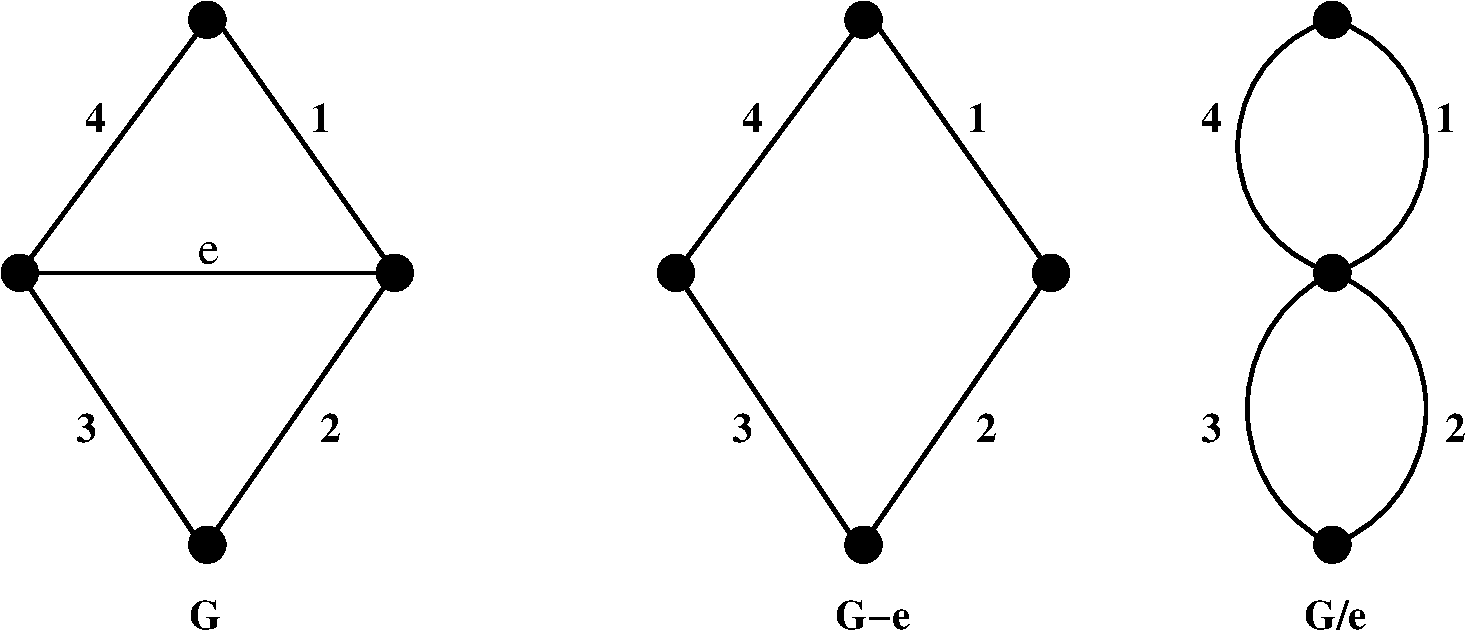
\includegraphics[width=10cm]{arboricity.pdf}
%% \caption{The arboricity polynomial does not satisfy a deletion contraction recursion.}
%% \end{figure}


%% \end{example}


%\subsection{Quasisymmetric Functions}

%I am assuming that we'll have this general theory set up earlier so I can just work through it in an example. 


%% ****cjk: I just wrote out examples but here we should explicitly describe arboricity in terms of the Erhart and Quasisymmetric picture.  I want to wait to do this until the other sections are written so we can point out specific results that apply.  Also, I actually don't like how all the examples are italized.****


%% \begin{example}

%% Consider the matroid of the $3$-cycle $M(C_3)$.  The only circuit is the entire ground set $\{1,2,3\}$.  All other ordered set partitions correspond to independent coverings of $C_3$: 
%% $$1|23, 2|13, 3|12, 1|2|3,$$
%% and all those with the order of the blocks permuted. 

%% Consider the braid arrangement in $R^3$, the ground set space of the
%% matroid, or edge set space of the graph.  These ordered set partitions
%% correspond to the collection of integer points which lie off of the
%% intersection: $x_1 = x_2 = x_3$.


%%  Hence the corresponding element of NCQSym is 

%% $${\bf{{\mathcal A}}}(M) = M_{(1|23)} + M_{(2|13)} + M_{(3|12)} + M_{(23|1)} + M_{(13|2)} +  M_{(12|3)} + $$ $$ M_{(1|2|3)} + M_{(1|3|2)}
%% + M_{(2|1|3)} + M_{(2|3|1)} + M_{(3|1|2)} + M_{(3|2|1)}. $$

%% \noindent Specializing under the type map we have an element of Qsym:

%% $${\mathcal A}(M) = 3 M_{(1,2)} + 3 M_{(2,1)} + 6 M_{(1,1,1)}. $$

%% \noindent Evaluating at ${\bf 1}^k $ we have the arboricity polynomial:

%% $$ A(M) = 3 { k \choose 2} + 3 { k \choose 2} + 6 { k \choose 3} = k^3 - k $$

%% \end{example}



 \bibliographystyle{amsplain}

 \bibliography{references}

\end{document}
